% Fundamental packages
\documentclass[11pt,a4paper,twoside]{book}
\usepackage[utf8]{inputenc}
\usepackage[american]{babel}
\usepackage{amsmath}
\usepackage{amsfonts}
\usepackage{amssymb}
\usepackage{graphicx}

% margins and general lay-out
%\usepackage[inner=3cm,outer=2cm,top=2.5cm,bottom=2.5cm]{geometry}
\usepackage[inner=2.5cm,outer=2.5cm,top=2.5cm,bottom=2.5cm]{geometry}
\pagestyle{plain}

% fonts (Helvetica) and typographical stuff 

\usepackage[T1]{fontenc}
\usepackage{lmodern} 
\usepackage{textcomp} 
\usepackage{pifont}
\usepackage{csquotes}
\usepackage{bm}

% Setting the font should be done after loading the typographic packages which tend to 
% set a new default font. The microtype package should however be loaded after the font ...
% using san serif helvetica clone
\usepackage{helvet}
\renewcommand{\familydefault}{\sfdefault}
% phv is another posibility.
% \renewcommand\rmdefault{phv}
\usepackage{microtype}

% additional packages
\usepackage{booktabs}
\usepackage{pdfpages}
\usepackage{hyperref}
\usepackage{float}
\usepackage{todonotes}
\usepackage{caption}
\usepackage{subcaption}
\usepackage{color}
\usepackage{multirow}

% package to manage citations
\usepackage[backend=bibtex,style=authoryear-comp,sorting=nyt,isbn=false,url=false, natbib=true]{biblatex}
\addbibresource{references.bib}

% Kill the auto-indent
\setlength\parindent{0pt}

% test package
\usepackage{lipsum}

% Packages for list of symbols and list of abbreviations
%\usepackage[nonumberlist,acronym,toc,nomain]{glossaries}
%\makeglossaries
%\input{Glossaries/Abbreviations}

% new definitions
\newcommand{\expit}{\text{expit}}
\newcommand*{\perm}[2]{{}^{#1}\!P_{#2}}%
\newcommand*{\comb}[2]{{}^{#1}C_{#2}}%
\newcommand*\diff{\mathop{}\!\mathrm{d}}
\DeclareMathOperator*{\argmax}{arg\,max}
\DeclareMathOperator*{\argmin}{arg\,min}

% start of the document
\begin{document}

% include cover page + copyright statement + no pagenumbers
\pagenumbering{gobble}
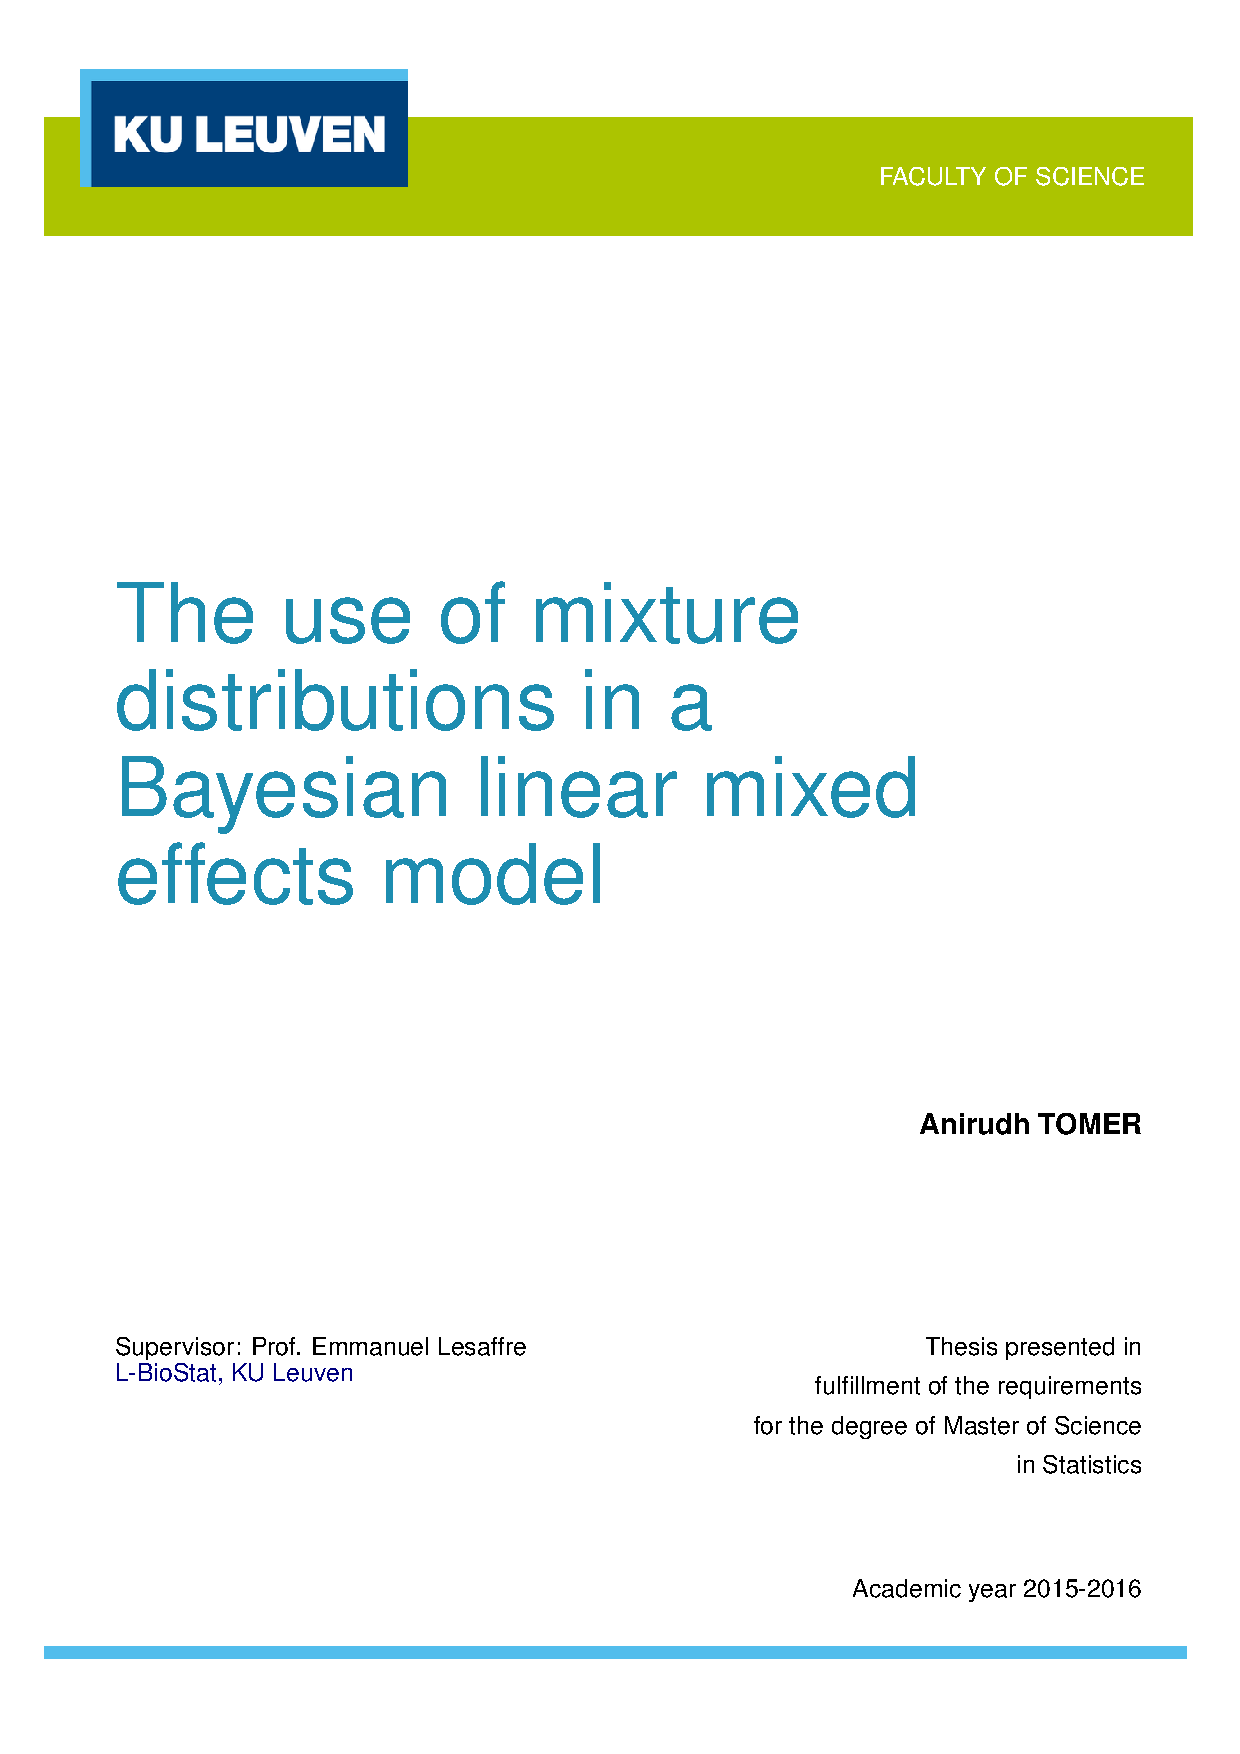
\includepdf[pages={1}]{coverpages/titlepage/titlepage.pdf}
%an empty page to make sure copyright gets printed on a new page
\clearpage \null \clearpage
\null
\vfill
\copyright~ Copyright by KU Leuven \\

Without written permission of the promotors and the authors it is forbidden to reproduce or adapt in any form or by any means any part of this publication. Requests for obtaining the right to reproduce or utilize parts of this publication should be addressed to KU Leuven, Faculteit Wetenschappen, Geel Huis, Kasteelpark Arenberg 11 bus 2100, 3001 Leuven (Heverlee), Telephone +32 16 32 14 01. \\

A written permission of the promotor is also required to use the methods, products, schematics and programs described in this work for industrial or commercial use, and for submitting this publication in scientific contests.
\cleardoublepage

% frontmatter + roman page numbers
\frontmatter

% !TEX root =  ../../thesis.tex

\chapter{Preface}
\label{ch : preface}

The following thesis work was conducted as part of the programme completion requirements of MSc. Statistics programme at KU Leuven. When I began working on this project, I had little idea that I would be able to go as far as I have been now. There were many significant obstacles on the way, such as analytical calculations of the various Deviance information criteria definitions, marginal likelihood, choice of posteerior predictive checks, implementating them in a software, Gibbs sampler idiosyncrasies and lack of computational power required for this work. However, at every step the work became more and more enticing. Looking backwards, I think it was one of the most interesting project I have done in recent times. Through and through, I enjoyed every bit of this project. The entire work for this thesis has been done using R and JAGS (Just Another Gibbs Sampler). The source code, results of simulations and an electronic draft of this thesis can be found at\\
\url{https://github.com/anirudhtomer/MScThesis}\\

In chapter 1 we present an introduction to mixture distribution and their central role in the formulation of the problem statement for this thesis. In Chapter 2 we present an introduction to the Bayesian paradigm as for the work of this thesis we use Bayesian methods. Futher in Chapter 3 we present the definition of a Bayesian heterogeneity model, and the issues with estimation of parameters in it. In Chapter 4 we present the formulae for various classes of Deviance information crieteria, marginal likelihood and posterior predictive checks that we used for model selection. Chapter 5 includes the results of the simulation study that was performed to check the efficacy of the aforemented Bayesian model selection methods. In chapter 6 we model the Blood donor data set \citep{nasserinejad_prevalence_2015} using a Bayesian heterogeneity model and use results from the simulation study to apply the right model selection criteria.\\

I am grateful to my supervisor Professor Dr. Emmanuel Lesaffre for keeping faith in my capabilities and for guiding me in the right direction. I enjoyed the fact that he never spoonfed me, yet was always available to discuss the difficult parts of the work at hand. He set very clear goals at the beginning of the year and continually monitored my progress thereafter. My interest in Bayesian statistics has grown by magnitudes under his supervision and I am looking forward to contribute more in this area. I would also like to extend my gratitude to Professor Geert Molenberghs and Professor Geert Verbeke for the captivating lectures on longitudinal data analysis. They introduced me to mixed models and empowered me with the tools of trade required to do the frequentist analysis of blood donor data set in this report. I am thankful to Kazem Nasserinejad from ErasmusMC for resolving many of my queries regarding the blood donor data set, and to Igor Milhoranca for providing the much needed inputs at crucial times. Lastly, I am grateful to my parents for the innumerable sacrifices they made to make sure I had as less obstacles as possible during my studies and I dedicate this work to them.\\

Anirudh Tomer\\
Leuven, Belgium\cleardoublepage
% !TEX root =  ../../thesis.tex

\chapter{Summary}
\label{ch : summary}

\todo[inline]{update the summary with the newest conclusions}

In this master thesis we fitted a finite mixture distribution for the random effects in a Bayesian linear mixed model. A mixture distribution for random effects allows to model the heterogeneity introduced by ignoring certain covariates in the mean structure of the model or to take into account the unknown non normal distriution for random effects. We then explored effectiveness of Bayesian model selection criteria (DIC, Bayes Factor, PPC) for choosing the number of component densities in the mixture distribution of random effects. Since mixture models are missing data models, we implemented various definitions of DIC as given by \citet{celeux_deviance_2006} for such models. We found that DIC 4 based on complete data likelihood was a fairly good selection criteria. However as the sample size decreased the discerning power of DIC also decreased. We then implemented Bayes Factor based on the approximation given by \citet{chib_marginal_1995} and found that it was not reliable for deciding on number of components required in the model. On the other hand, Posterior predictive checks were a very strong discerning method if indepdent inverse gamma priors were used for variance components, and uniform distribution for correlation, in the distribution of random effects. In regards to the choice of prior distribution for covariance parameters, we found that a Wishart prior for precision matrix(inverse of covariance matrix) overestimates the precision when within subject variance is greater than between subject variance. Thus, it could be a good idea to decrease scale of the intercept and the covariate corresponding to random slope, so that the corresponding variances increase in magnitude.
%\printglossary[type=\acronymtype,style=list,title={List of abbreviations}]
\cleardoublepage
\tableofcontents
\listoftables
\cleardoublepage
\listoffigures
\cleardoublepage

% main matter (chapters + appendices
\mainmatter
% !TEX root =  ../../thesis.tex 

\chapter{Introduction}
\label{ch : introduction}

In this chapter we will first introduce the mixture distribution and then mention the challenges involved in estimation of parameters of a mixture distribution. We will also highlight the benefits of using a Bayesian approach for parameter estimation. Lastly we will present the goal of this master thesis, in which a mixture distribution plays the central role.

\section{Mixture distribution}
\label{sec : mixture_distribution}
A mixture distribution is a probability distribution of a random variable formed from a group of other random variables. The formation of a mixture distribution can be seen as a two step process, in which firstly a particular random variable is selected from a collection of random variables based on a certain probability of selection. In the second step a value is sampled for the selected random variable from its probability distribution. For e.g. the following random variable $Y$ has a mixture density formed from 3 normally distributed random variables.

$$Y \sim \dfrac{1}{6}N(-10,3) + \dfrac{1}{2}N(0,1) + \dfrac{1}{3}N(4,2)$$

\begin{figure}
	\centering
	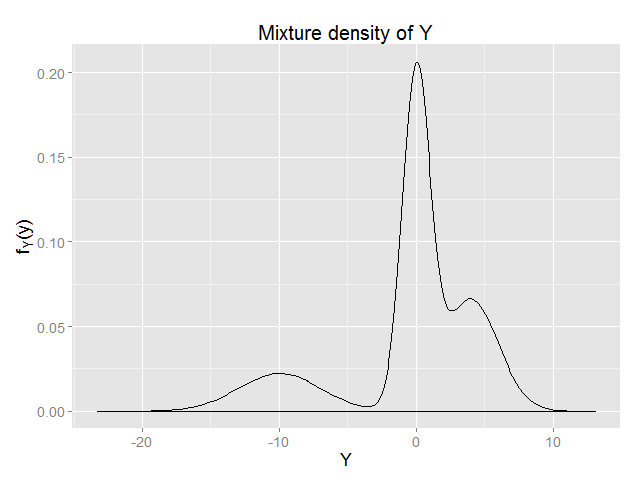
\includegraphics[scale=0.5]{mainmatter/chapter_1_introduction/mixture_density.png}
	\caption{Mixture density of $Y \sim \dfrac{1}{6}N(-10,3) + \dfrac{1}{2}N(0,1) + \dfrac{1}{3}N(4,2)$}
	\label{fig : mixture_density_1}
\end{figure}

Figure \ref{fig : mixture_density_1} shows the density function for $Y$. The density is trimodal with each mode corresponding to one of the components in the mixture. Mixtures like $Y$ which are formed from a finite sum of components are called finite mixtures. The components are also known as mixture components and their densities are called component densities. The constants multiplying the corresponding densities are called mixture weights. The mixture weights also represent the probability of selection of each component density. Each mixture weight should be positive and the sum of all mixture weights should be equal to 1. While in our example all the  mixture components were having the same parametric family i.e. Normal distribution, it is also possible to have mixture components from different parametric families. A mixture model where it is assumed that all data points are generated from a mixture of normally distributed component densities is called Gaussian mixture model (GMM). It is important to note that the idea of a mixture distribution is rather hypothetical, as in an example by \citet{titterington_statistical_1986} it was shown that a GMM of two components could be indistinguishable from a log-normal distribution.

\subsection{Formal definition for finite mixture distribution}
\label{subsec : formal_def_mixture_dist}
Given a finite set of $K$ probability density functions $p_1(y), p_2(y), \ldots, p_K(y)$ and weights $\eta_1, \eta_2, \ldots, \eta_K$, a random variable $Y$ is said to have a finite mixture distribution if

$$p(y) = \sum_{k=1}^{K} \eta_{k} p_{k}(y)$$

The vector of the weights $\boldsymbol{\eta} = (\eta_1, \eta_2, \ldots, \eta_K)^T$ is called the weight distribution. The $k^\text{th}$ weight $\eta_{k}$ corresponds to selection probability of the $k^\text{th}$ density while sampling for $Y$. It can only take values from the $K$ dimensional positive real coordinate space ${\mathbb{R}^{+}}^K$ with an additional constraint, $\sum_{k=1}^{K} \eta_{k} = 1$.\\

\subsection{Challenges}
\label{subsec : challenges_mixture_density}
The primary challenge while modeling a mixture density for a random variable is that the number of mixture components ($K$), weight distribution $\boldsymbol{\eta}$ and the corresponding parameters for component densities are rarely known in advance. Secondly, from a sample of $N$ observations $y_1, y_2, \ldots, y_N$ sampled from the mixture density $p(y)$ one may not know which observation belongs to which component density. Formally, an allocation vector $\boldsymbol{S} = (S_1, S_2, \ldots, S_N)^T$ represents the allocation of observations to mixture components. i.e. $S_i = k$ represents that $i^\text{th}$ observation belongs to $k^\text{th}$ component density. Estimating the allocation vector is in fact solving the clustering problem, albeit using parametric methods in our case.\\

While Maximum Likelihood based methods such as the EM algorithm could be used to deal with the above mentioned challenges, there are certain downsides to them. Firstly it is well known that 95\% confidence intervals of ML estimates are based on asymptotic normality of the estimators. Thus in case of small sample size, or small mixture weights the results will not be correct \citep[pg. 35]{fruhwirth-schnatter_finite_2013}. A Bayesian approach however is immune to these issues as the posterior distribution of parameters is allowed to be non-normal. Secondly, in case of univariate and multivariate GMM, the likelihood function

$$ p(\boldsymbol{y}|\boldsymbol{\mu}, \boldsymbol{\sigma^2}, \boldsymbol{\eta}) = \prod_{i=1}^{N} \sum_{k=1}^{K} f_N(y_i; \mu_k, \sigma^2_k) \eta_k$$

is unbounded and has many spurious nodes near the boundary of the parameter space for variance($\sigma^2_k$) of the components \citep{kiefer_consistency_1956,day_estimating_1969}. A Bayesian approach however, handles this problem elegantly using priors for parameters of the component densities. For e.g. \citet[pg. 176]{fruhwirth-schnatter_finite_2013} combined the likelihood with the prior $p(\mu_k, \sigma^2_k) \propto p(\sigma^2_k), \sigma^2_k\sim \text{Inv-Gamma}(1,4)$, and showed that it lead to a joint posterior density $p(\mu, \sigma^2 | \boldsymbol{y})$ of parameters in which $\sigma^2_k$ was bounded away from 0. Thus all the spurious nodes near the boundary of the parameter space for $\sigma^2_k$ were cut out, whereas they were apparent for the surface of the likelihood function.

\subsection{Applications of mixture distributions}
Mixture models have found usage in a variety of domains. Some of the examples are:
\begin{itemize}
\item Spike sorting of neural data: Both GMM and mixture of multivariate t-distributions have been used.\citep{lewicki_bayesian_1994,shoham_robust_2003}.
\item Speaker recognition as well as speech to text conversion algorithms have used mixture models \citep{simancas-acevedo_speaker_2001,xiang_efficient_2003,povey_subspace_2011}.
\item Image processing: GMM have been used to find features in an image, such as objects, boundaries etc. \citep{fu_color_2012}. For e.g. \citet{ming-hsuan_yang_gaussian_1998} have used GMM to model the distribution of skin color pixels. Many authors have also proposed using GMM for face recognition. i.e. as a biometric identification mechanism.
\item Finance: \citet{brigo_lognormal-mixture_2002} proposed to use a log-normal mixture distribution for pricing of financial assets.
\item Biology: Mixture models have found usage in genetics and cell biology.\citep{sim_evaluating_2012,gianola_mixture_2007} 
\end{itemize}

The example applications we cited involved usage of mixture models to adjust for a hidden attribute in the data which could not be collected or to approximate a density which is not of known form. However mixtures have also been used as supplementary methodology in various models, a list of which can be found in \citet[pg. 238]{fruhwirth-schnatter_finite_2013}. One such usage in linear mixed models has been proposed by \citet{verbeke_linear_1996} and it also forms the theme of this thesis.

\section{Goal of master thesis}
\label{sec : goal}
\citet*{verbeke_linear_1996} proposed to use a finite mixture distribution of normally distributed components for the prior distribution of random effects in a linear mixed effects model (LMM). This particular LMM is also known as Heterogeneity model. For the scope of this thesis our focus will be on the Bayesian version of the linear mixed effects model(BLMM), where all parameters involved are assigned a probability distribution. Needless to say, the issues described in section \ref{subsec : challenges_mixture_density} are also applicable for the Bayesian heterogeneity model. The aim of this master thesis is to evaluate existing Bayesian approaches for model selection, namely Deviance Information Criterion (DIC) , marginal likelihood and posterior predictive checks(PPC) for selecting the right number of mixture components for the distribution of random effects. Since we will be working in the Bayesian framework, we will use MCMC methods instead of the frequentist point estimation methods. We will simulate data sets to check efficacy of each of the aforementioned model selection criteria and then use the most effective ones to decide the number of mixture components for the random effects distribution in Blood donor longitudinal data set \citep{nasserinejad_prevalence_2015}.
% !TEX root =  ../../thesis.tex 

\chapter{Bayesian paradigm}
\label{ch : bayesian_paradigm}

\section{The bayesian motivation: A toy example}
To explain the motivation behind the bayesian paradigm, we will use an informal approach via the following toy example. Suppose there are three people A,B and C of whom A and B each are captains of a cricket team and C is the refree who tosses the coin. Given the importance of the toss in this sport each side would like to win the toss. Let us assume that based on experiences of an old friend captain B gets to know that the referee purposefully attempts at getting a heads on the toss. However given the nature of this problem, it is hard to quantify this belief in a single real number. Instead a belief that there is a 70 to 90\% chance that the result will be a heads is more likely than a belief that there is exactly an 80\% chance for the same. One might also have a slightly vague belief that there is more than 50\% chance that the toss will result into a heads. \\

\begin{figure}
\centering
	\begin{subfigure}[b]{0.45\textwidth}
		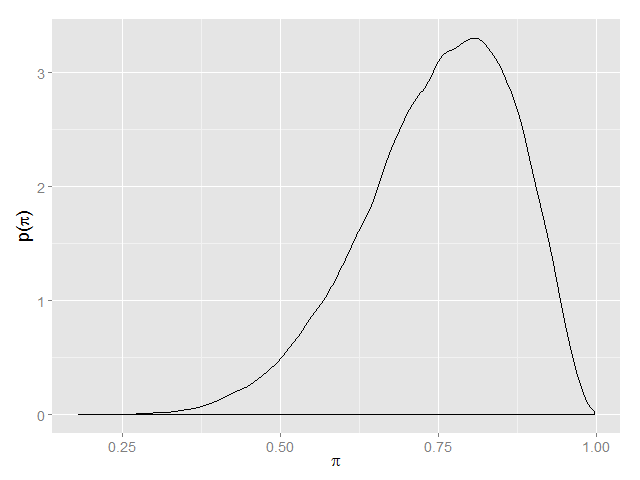
\includegraphics[width=\textwidth]{mainmatter/chapter_2_bayesian_paradigm/beta_prior.png}
        \caption{Prior $p(\pi)$: $\beta(9,3)$}
        \label{subfig : toy_problem_prior}
	\end{subfigure}
    	\begin{subfigure}[b]{0.45\textwidth}
		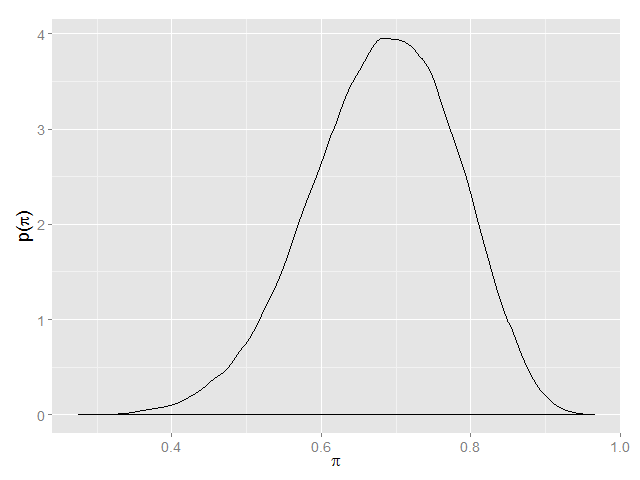
\includegraphics[width=\textwidth]{mainmatter/chapter_2_bayesian_paradigm/beta_posterior.png}
        \caption{Posterior $p(\pi|\boldsymbol{y})$: $\beta(15,7)$}
        \label{subfig : toy_problem_posterior}
	\end{subfigure}
\caption{Prior and posterior PDF for $\pi$; the probability of getting heads.}
\end{figure}

While subjective, these beliefs represent the prior probability distribution of a random variable in bayesian paradigm. In our toy problem the random variable is probability $\pi$ of getting a heads. For e.g. in figure \ref{subfig : toy_problem_prior} we can see one such prior distribution corresponding to the belief that the chance of getting a heads on toss is more than tails and it is more likely to be somewhere between 70 to 90\%. This is in contrast to the frequentist paradigm where parameters do not have a distribution but are rather constants. Also the point and interval estimation in frequentist paradigm do not take prior beliefs into account and rely completely on the data at hand. While a detailed discussion of Bayesian vs. Frequentist approaches can be found in \citet{lesaffre_bayesian_2012}, we will present a brief overview of Bayes theorem and its usage in bayesian parameter estimation.\\

\section{Bayes theorem}
\label{sec : bayes_theorem}
To understand the use of Bayes theorem in parameter estimation let us first look at one of the frequentist approach Maximum likelihood estimation to estimate the probability of getting heads ($\pi$). Suppose after 10 matches captain B observed that 6 times out 10 the toss resulted in heads. Assuming that conditions in each toss were such that the tosses were independent, then based on the likelihood function $L(\pi|\boldsymbol{y})$ the MLE of $\pi$ will be $\hat{\pi} = 0.6$. In contrast, the Bayes rule provides the framework to estimate the entire distribution of $\pi$ based on the data and the prior beliefs. The bayes rule for the continuous parameter $\pi$ is given by\\

\begin{equation}
\label{eq : bayes_rule}
p(\pi|\boldsymbol{y}) = \dfrac{L(\pi|\boldsymbol{y})p(\pi)}{p(\boldsymbol{y})} = \dfrac{L(\pi|\boldsymbol{y})p(\pi)}{\int_{0}^{1}L(\pi|\boldsymbol{y})p(\pi)d\pi}
\end{equation}

The result $p(\pi|\boldsymbol{y})$ is called the posterior distribution of the parameter based on which statistical inference about the parameter can be done. An intuitive way to get the motivation behind the bayes theorem is that the denominator can be seen as marginal probability of $\boldsymbol{y}$ based on the law of total probability. This is more evident in the categorical case though. In figure \ref{subfig : toy_problem_posterior} we can see the posterior PDF for the probability of getting heads that we obtained after applying Bayes rule. The mean value of this distribution is 0.7 which if you compare with the MLE of 0.6 you can see that bayesian posterior mean is influenced by the prior as well.\\
\todo[inline]{The intuition part is needed to be expanded upon, and shall I talk of CI at this moment???}

\section{Bayesian software}
We can see in equation \ref{eq : bayes_rule} that the computation of posterior involves solving the integral in the denominator. While the calculations are simple in certain cases, for e.g. in exponential family the choice of conjugate prior leads to a posterior belonging to the same family. However it also depends on the prior beliefs. For e.g. if the prior belief for $\pi$ in our toy example is that it is trimodal then we may have to use numerical approximation for calculation of the posterior. The most widely used algorithms for posterior approximation are Markov chain monte carlo (MCMC) techniques like Gibbs sampling, Slice sampling, Metropolis hastings and their variants etc.\\

The software tools we will use are from the BUGS family like JAGS or WinBUGS. While WinBUGS provides its own integrated development environment it definitely lacks the usability and visualization capabilities offered in R. JAGS on the other hand relies on third party tools completely for visualization and analysis of MCMC chains. There are R packages namely R2jags, R2WinBUGS which allow users to execute JAGS/WinBUGS code via R. For bayesian linear mixed models the R package blme will be used. For bayesian mixture models we will evaluate the R package bayesmix. The R package coda provides a rich array of functions to do analysis and diagnosis of MCMC chains.\\
% !TEX root =  ../../thesis.tex

\chapter{Bayesian linear mixed effects model}
\label{ch : blmm}

\section{Introduction to linear mixed model}
\label{sec : lmm}
A linear mixed effects model, also known as linear mixed model(LMM) is a statistical model for data which is hierarchical in structure. The specialty of the models is that apart from the fixed effects, they also model the correlation between the observations falling in the same group at a certain level in the hierarchy. The correlation is modeled with the help of random effects and the response is modeled as a linear function of both fixed and random effects.\\

There are many synonymous terminologies for data sets which are hierarchical in nature albeit with subtle nuances differentiating them. In this thesis our focus will be on Longitudinal data sets. A longitudinal data set is the one where multiple observations are collected from subjects at different points in time. For e.g. measurement of Hemoglobin of 20 patients with observations taken every month for a period of 24 months. Since the observations collected from a subject will be correlated a linear model will not be useful because of the restrictions it imposes on the covariance structure.\\

\todo[inline]{Should I mention that Laird and Ware proposed the model?}

\subsection{LMM definition}
\label{subsec : lmm_definition}
Following the notations from \citet{lesaffre_bayesian_2012}, the LMM for the observations of the $i^{th}$ subject among the $n$ subjects is given by\\

$$\boldsymbol{y_i} = \boldsymbol{X}_{i}\boldsymbol{\beta} + \boldsymbol{Z}_{i}\boldsymbol{b}_{i} + \boldsymbol{\varepsilon}_{i}$$\\

where $1 \le i \le n$,\\
$\boldsymbol{y}_i = {(y_{i1}, y_{i2}, \ldots, y_{im_i})}^T$ is a vector of observations for the $i^{th}$ subject taken at $m_i$ time points,\\
$\boldsymbol{X}_i = {(\boldsymbol{x}_{i1}^T, \boldsymbol{x}_{i2}^T, \ldots, \boldsymbol{x}_{im_i}^T)}^T$ is the $m_i \times (d+1)$ design matrix for the $i^{th}$ subject,\\
$\boldsymbol{\beta} = {(\beta_0, \beta_1, \ldots, \beta_d)}^T$ is a $(d+1) \times 1$ vector of fixed effects with $\beta_0$ being the intercept,\\
$\boldsymbol{Z}_i = {(\boldsymbol{z}_{i1}^T, \boldsymbol{z}_{i2}^T, \ldots, \boldsymbol{z}_{im_i}^T)}^T$ is the $m_i \times q$ design matrix of covariates varying for a subject at each observation,\\
$\boldsymbol{b}_i = {(b_{0i}, b_{1i}, \ldots, b_{(q-1)i})}^T$ is a $q \times 1$ vector of random effects with $b_{0i}$ being the random intercept. The random effects $\boldsymbol{b}_i \sim N_q(\boldsymbol{0}, G)$ with $G$ being the $q \times q$ covariance matrix,\\ 
$\boldsymbol{\varepsilon}_{i} = {(\varepsilon_{i1}, \varepsilon_{i2}, \ldots, \varepsilon_{im_i})}^T$ is a $m_i \times 1$ vector of measurement errors. The errors $\boldsymbol{\varepsilon}_{i} \sim N_{m_i}(\boldsymbol{0}, R_i)$ with $R_i$ being the $(m_i \times m_i)$ covariance matrix of errors,\\

The errors $\boldsymbol{\varepsilon}_{i}$ and the random effects $\boldsymbol{b_i}$ are assumed to be independent. $R_i$ is usually a diagonal matrix of the form $\sigma^2I_{m_i}$. While one might only model the correlation between the observations of a subject using random effects, it is also possible to model the serial correlation component. For this and an in depth coverage of LMM we refer the reader to \citet{verbeke_linear_2009}.\\

\section{Motivation for Bayesian linear mixed model}
\label{sec : blmm}
One of issues with the frequentist LMM is that while the parameters in matrices $G$ and $R_i$ are estimated using ML/REML only a point estimate is further used in estimation of fixed effects(see \cite[chap. 5]{verbeke_linear_2009}). Hence the uncertainty in estimation of random effects is ignored. Although frequentist inference approaches try to mitigate this issue by modifying the distributional assumptions of the test statistic \citep[pg. 56]{verbeke_linear_2009}, a bayesian approach considers the variability in parameter estimates in the first place. A similar problem occurs in the estimation of $\boldsymbol{b_i}$. The frequentist strategy is to use Empirical bayes estimates where the the posterior distribution of random effects uses point estimates of parameters in matrices $G$ and $R_i$. Thus the uncertainty in estimation is ignored. On the other hand the bayesian approach averages out over the entire posterior distribution of the hyperparameters to obtain the posterior $p(\boldsymbol{b_i}|\boldsymbol{y})$. In light of these reasons, in this thesis we will model our data using Bayesian linear mixed models.\\

The Bayesian linear mixed model or BLMM can be obtained by assigning a distribution to all the parameters involved in a LMM. This means that for the model presented in section \ref{subsec : lmm_definition} we will have a prior distribution for the following:
\begin{itemize}
\item $\sigma^2 \sim p(\sigma^2)$
\item $\boldsymbol{\beta} \sim p(\boldsymbol{\beta})$
\item $G \sim p(G)$
\end{itemize}

\section{Motivation for mixture of random effects}
As we saw above the random effects are assumed to be multivariate normally distributed. It could be too strong an assumption though in certain cases. A classical example of it are the longitudinal studies where at any time point we would like to categorize subjects in groups. For e.g. group with a high risk of having a certain disease in future vs. group with a low risk. While in retrospective studies it is quite easy as we know exactly which patients were diagnosed with the disease and which were not. However in a study where we would like to categorize patients into different groups well before diagnosis this could be difficult. Here is a toy example for it. Imagine that in longitudinal study we are measuring a response $Y$ which is an indicator of a disease. Assume that from a previous study it is known that patients which are in high risk group for the disease tend to have a higher response $Y$ during all times. Also assume that the trend of $Y$ over time remains the same for both groups otherwise. Figure \ref{fig : random_slope_dummy_data} shows individual profiles of subjects from a simulated dataset. Looking at this plot we can say that a random intercept component will be enough to model individual profiles. Since we will not be knowing which patient belongs to which group, this heterogeneity can be appropriately modeled by considering that the random intercept is a mixture of two normal components.\\

\begin{figure}
	\centering
	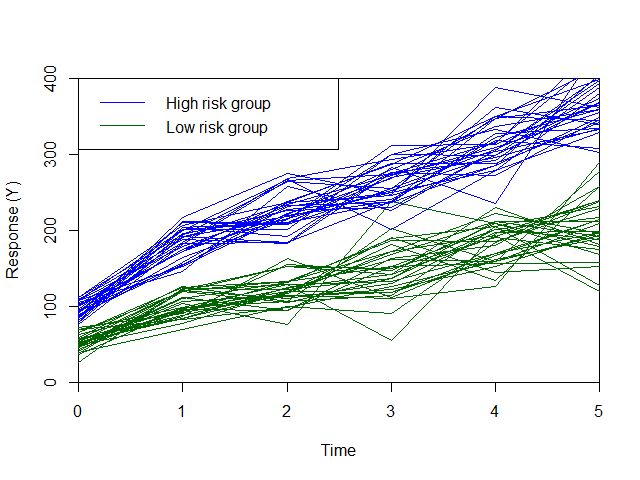
\includegraphics[scale=0.5]{mainmatter/chapter_3_blmm/random_slope_dummy_data.png}
	\caption{Individual profiles of 30 subjects from each group.}
	\label{fig : random_slope_dummy_data}
\end{figure}

In a LMM is quite common to use histogram of Empirical Bayes estimates of random effects to detect groups of individuals. However \citet{verbeke_linear_1996} have shown that if the prior is misspecified(for e.g. if in our example we use a single normal distribution), then it is possible that the histogram of estimates of random effects will be shrunk towards the prior distribution. This means that in our case we may not see a histogram with two distinct modes. The model where a mixture of Gaussian components were used to specify the random effects distribution is called a Heterogeneity model. Various applications of the heterogeneity model can be found in \citet[pg. 264]{fruhwirth-schnatter_finite_2013}.\\

\subsection{Mathematical notation}
Since the random effects are having a Gaussian mixture distribution we will use the following notation to express it mathematically.\\

$$\boldsymbol{b}_i \sim \sum_{k=1}^{K} \eta_k N_q(\boldsymbol{b}_k^C, G_k)$$\\
where $\boldsymbol{b}_k^C$ and $G_k$ are the mean vector and covariance matrices for the $k^{th}$ component in the mixture distribution respectively. The vector $\boldsymbol{\eta} = (\eta_1, \eta_2, \ldots, \eta_K)$ is the weight distribution for the component densities. Since we are following the bayesian paradigm, in addition to prior distribution for $\boldsymbol{\beta}$ and $\sigma^2$ we will now have prior for ($\boldsymbol{b}_1^C, \boldsymbol{b}_2^C, \ldots, \boldsymbol{b}_K^C, \boldsymbol{\eta}, G_1, G_2, \ldots, G_K$).

\section{Parametrization in BLMM}
The random effects $\boldsymbol{b}_i$ in a mixed model could be seen as random deviations from the fixed effects($\boldsymbol{\beta}$) with a mean $\boldsymbol{0}$. For a longitudinal data set, it means that the overall effect of a covariate like time for a subject should be the sum of both fixed and random effects. In this case matrices $\boldsymbol{X}$ and $\boldsymbol{Z}$ both share columns corresponding to the variable time. To enforce the mean $\boldsymbol{0}$ on the random effects in a mixture distribution the following condition should be satisfied.\\

$$E(\boldsymbol{b}_i | \boldsymbol{\phi}) = \sum_{k=1}^{K} \eta_k N_q(\boldsymbol{b}_k^C, G_k) = 0$$,\\
where $\boldsymbol{\phi}$ is the vector ($\boldsymbol{b}_1^C, \boldsymbol{b}_2^C, \ldots, \boldsymbol{b}_K^C, \boldsymbol{\eta}, G_1, G_2, \ldots, G_K$). This further means that $E(\boldsymbol{y}_i | \boldsymbol{\phi}) = \boldsymbol{X}_{i}\boldsymbol{\beta}$. This parametrization which was also used in the original paper on Heterogeneity model \citep{verbeke_linear_1996} is called noncentralized parametrization. The centralized parametrization assumes that the random effects are not deviations from the fixed effects and are centred around a non zero mean. The choice of parametrization has an effect on the rate of convergence while estimating parameters using MCMC. The non-centralized parametrization could be used when within subject heterogeneity is considerably smaller than the heterogeneity due to random effects. Otherwise a centralized parametrization is preferred. We refer the reader to \citet{fruhwirth-schnatter_bayesian_2004} for further details.

\section{Likelihood: Complete data vs Mixture}
The likelihood function in a mixture distribution depends on how much we know about the data. If we know both the data and the allocation vector $\boldsymbol{S}$ then the following likelihood function of parameters is called a complete data likelihood function.\\
$$p(\boldsymbol{y, S}|\boldsymbol{\nu}) = \prod_{i=1}^{N} \prod_{k=1}^{K} (p(\boldsymbol{y}_i | \boldsymbol{\theta}_k) \eta_k)^{I_{S_i=k}}$$\\
where $\boldsymbol{\nu} = (\boldsymbol{\theta}_1, \boldsymbol{\theta}_2, \ldots, \boldsymbol{\theta}_K, \boldsymbol{\eta})$ is a vector of weight distribution and parameters of component densities. It is possible to write this complete data likelihood function in $\perm{K}{K} = K!$ equivalent ways by permuting the order of components. Each order of components is called a Labeling scheme. Although this idea seems trivial we will see ahead that it creates a problem during estimation called label switching. While this likelihood function is valid conditional on knowing the allocation vector $\boldsymbol{S}$, the following likelihood function called Mixture likelihood function applies when we are not aware of the allocations.\\

$$p(\boldsymbol{y}|\boldsymbol{\nu}) = \prod_{i=1}^{N} (\sum_{k=1}^{K} p(\boldsymbol{y}_i | \boldsymbol{\theta}_k) \eta_k)$$\\

It is interesting to note that the mixture likelihood function is symmetrical and has $K!$ modes. We refer readers to \citet[pg. 45-46]{fruhwirth-schnatter_finite_2013} for the review of geometric presentation of this likelihood function.\\

\section{Mixture model identifiability: Label switching}
After running a MCMC procedure to estimate the posterior distributions of the parameters involved, we will be interested in knowing the parameters for the component densities. In most cases we will also be interested in classification of observation using allocation probabilities $P(S_i = k | \boldsymbol{y})$. Now let us imagine that we fitted exactly the true number of components ($K^{true}$ from which the mixture density was formed. At this point it is possible that the posterior densities of parameters do not reflect the true posterior distribution due to label switching.\\

To idea of label switching could be explained with this simple example. Suppose we have a mixture distribution $0.5N(5,1) + 0.5N(7,1)$of two components $C_1$ and $C_2$ and we sampled a few observations from it. The MCMC procedure we will estimate parameters using data augmentation. i.e. we begin with some random allocation vector $\boldsymbol{S}^0$ and estimate parameters using complete data likelihood. For MCMC labels $\mu_1$ and $\mu_2$ exist rather than  $\mu_{C1}$ and $\mu_{C2}$ and it does not associate labels with actual components. We begin with a vague joint prior for these parameters $p(\mu_1, \mu_2) = p(\mu_1)*p(\mu_2) = p(\mu_1)*p(\mu_1) = p(\mu_2)*p(\mu_2)$.\\

Assume that the allocation vector we began with assigns all observations from component $C_1$ to label 1 and all observations from component $C_2$ to label 2. Under such a scheme $(\mu_1,\mu_2) = (5,7)$ is likely. However if we take a conjugate of this allocation vector $(\mu_1,\mu_2) = (7,5)$ will also be accepted. This because we have a mixture likelihood function which is bimodal. Now let us imagine a scenario where because of our initial allocation vector, parameter estimates are $(\mu_1, \mu_2) = (5.5,6.5)$. So far it seems $\mu_1$ represents $\mu_{C1}$ and $\mu_2$ represents $\mu_{C2}$. Now we estimate allocation vector conditional on these estimates in MCMC. Supposing that an observation with value 6.5 originally from component $C_2$ gets allocated to component $C_1$ and similarly an observation with value 5.5 from component $C_1$ gets allocated to $C_2$. Unless we impose some constraint like $\mu_1 < \mu_2$, under the current situations even $(\mu_1,\mu_2) = (6.5, 5.5)$ could be sampled by MCMC. This because under the mixture likelihood it is also likely. However this scenario could've been unlikely if the true means were very far apart. In our scenario the issue is that posterior for $\mu_1$ will have a multiple modes. Not only that but if the sampler kept on arbitrarily switching between the two equivalent posterior regions then both regions will be partially explored. Thus any inference based on this posterior will be useless. \citet[pg. 82]{fruhwirth-schnatter_finite_2013} suggest to use a balanced label switching, which gives multimodal posterior albeit with a full exploration.\\

It is interesting that if our prior for the parameters was not vague, but exactly equal to the true distribution of parameters then label switching might not have happened. However the problem with a strong prior is that an incorrect strong prior could also inadvertently cause label switching or it might not allow a complete exploration of the posterior. Other techniques to stop label switching are imposing an identifiability constraint, which in our case was $\mu_1 < \mu_2$. However in higher dimensions it could become difficult to find a constraint which imposes a unique labeling scheme. For more details we refer the reader to \citet{stephens_dealing_2000}.\\

\section{Mixture model identifiability: Equal or empty components}
A mixture model will also be unidentified if we have an empty component or two components with the same parameters. Suppose the true number of components is $K^{true}$ and we fit $K = K^{true} + 1$ components. In the MCMC sampler suppose one of the components is assigned any observation. Thus the posterior for the parameters will remain the same as the prior. Assuming that the prior for weight distribution $\boldsymbol{\eta}$was a Dirichlet prior $\mathcal{D}(0.5, 0.5, \ldots, 0.5)$, then we will have a posterior for $\boldsymbol{\eta}$ such that the $K^{th}$ component will always have an almost 0 weight in the mixture distribution. This means that at the end of MCMC sampling the component density's posterior will be same as its prior and no observations will be allocated to the component. In such cases the true number of components could be estimated by the count of components with non zero number of allocations. However this situation could be avoided with a stronger prior on the weight distribution which forces the posterior distribution of $\boldsymbol{\eta}$ to be such that no components are empty at the end of MCMC sampling. Identification of number of components in such case is explained in the next section.\\

\textcolor{red}{Gosh! I should explain it in terms of pulling away the posterior eta from the boundary where components of eta are linearly dependent.}. 

\todo[inline]{Should I also discuss the choice of prior?}

\section{Choosing the right number of mixture components}
In most cases we do not know the right number of mixture components in advance unless we have some expert knowledge available or we know them from a previous/similar study. As part of this thesis we will compare many of the existing methods for finding the right number of mixture components.\\

\subsection{Information criteria based methods}
Information criteria are used to select models with parimony and good predictive power. Some of information criteria proposed in the literature are AIC proposed by Akaike, BIC (a minor modification of Schwarz's original criteria), DIC. While AIC and BIC are primarily used in frequentist statistics as they use point estimates of the parameters, DIC follows a more bayesian approach. Following are the definitions of the three criteria:\\

\begin{itemize}
\item $AIC = -2log(p(\boldsymbol{y}|\boldsymbol{\hat{\theta}})) + 2p$
\item $BIC = -2log(p(\boldsymbol{y}|\boldsymbol{\hat{\theta}})) + log(N)p$
\item $DIC = -2log(p(\boldsymbol{y}|\boldsymbol{\bar{\theta}})) + 2p_{DIC}$\\
where $\boldsymbol{\bar{\theta}} = E(\boldsymbol{\theta}_{post}|\boldsymbol{y})$,\\
$p_{DIC} = -2(E(log(p(\boldsymbol{y}|\boldsymbol{\theta}_{post}))) - log(p(\boldsymbol{y}|\boldsymbol{\bar{\theta}})))$ is the penalty for model complexity.
\end{itemize}

It is interesting to mention that the hierarchical nature of the mixture model implies a marginal model as well, which can be found by integrating out the random effects. \citet{verbeke_linear_1996} in their paper on heterogeneity model estimate the fixed effects and all covariance components using this marginal model. In our case y has a marginal model given by:\\

$$\boldsymbol{y_i} \sim \sum_{k=1}^{K} \eta_k N(\boldsymbol{X}_{i}\boldsymbol{\beta} + \boldsymbol{Z}_{i}\boldsymbol{b}_k^C,\boldsymbol{Z}_{i}G_{\boldsymbol{S}_i}\boldsymbol{Z}_{i}^T + R_i)$$\\

If our likelihood function is based on the marginal model then DIC could be used to select models which have good predictive power for an observation which is not necessarily from a subject who is in the current study. The total number of terms which will be penalized by AIC is equal to $dim(\boldsymbol{\eta}) + dim(\boldsymbol{\beta}) + dim(\boldsymbol{b}_{1}^C) + \ldots + dim(\boldsymbol{b}_{K}^C) + dim(G_1) + \ldots + dim(G_K) + 1(for \sigma^2)$, where dim is the total number of elements in the vector or matrix. On the other hand if we stick to the hierarchical interpretation, then DIC could be used to select models which have good predictive power for an observation which has to be from the current set of subjects. The total number of terms which will be penalized by AIC is equal to $dim(\boldsymbol{\beta}) + dim(\boldsymbol{b}_1) + \ldots + dim(\boldsymbol{b}_n) + 1(for \sigma^2)$. A model.

\subsection{Trans Dimensional Bayesian inference}
To compare a set of competing models $\mathcal{M}_1, \mathcal{M}_2, \ldots, \mathcal{M}_{K_{max}}$ each with their own set of parameters $\boldsymbol{\nu}_1, \boldsymbol{\nu}_2, \ldots, \boldsymbol{\nu}_{K_{max}}$ trans dimensional MCMC methods can be used. For e.g. Product space MCMC methods try to simultaneously sample the posterior probability $p(\mathcal{M}_{k}, \boldsymbol{\nu}_1, \boldsymbol{\nu}_2, \ldots, \boldsymbol{\nu}_{K_{max}}, \boldsymbol{y}$ for all $K_{max}$ models. The idea is that during each run a model indicator $\mathcal{M}$ which could follow for e.g. a multinomial distribution, is sampled. Suppose the model indicator is $M=2$ then all the parameters $\boldsymbol{\nu_{2}}$ are sampled whereas parameters for other models are kept what they were. The marginal posterior probability $p(\mathcal{M}_k|\boldsymbol{y}$ of the $k^{th}$ model is found by integrating out the parameters from the joint posterior. These could be further compared to select one of the K models.\\

\subsubsection{Marginal likelihood}
The ratio of marginal posterior could also be expressed as a Bayes Factor (assuming the prior probabilities for both models are equal) which is a ratio of Marginal likelihoods $\dfrac{p(\boldsymbol{y}|\mathcal{M}_i}{p(\boldsymbol{y}|\mathcal{M}_j}$ for the models. 
However \citet{johannes_berkhof_bayesian_2003} also suggest to use goodness of fit measures to be used along with Bayes factor. This because bayes factor is a relative measure. Relying on it completely could lead to selection of a model which is relatively better but overall does not provide a good fit.

\subsection{Posterior predictive checks}


\subsection{Other methods}
We will also explore other graphical methods or informal methods like method of moments in this thesis. For further reading on them we refer the reader to \citet[pg. 107-114]{fruhwirth-schnatter_finite_2013}
% !TEX root =  ../../thesis.tex
\chapter{Model selection criteria}
\label{ch : model_selection}

In most cases we do not know the right number of components in a mixture distribution in advance. As part of this thesis we will compare 3 of the existing Bayesian methods for finding the right number of mixture components.

\section{Deviance information criteria}
\label{sec : dic}

The Deviance information criteria or DIC was first proposed by \citet{spiegelhalter_bayesian_2002} for Bayesian model selection. The motivation for DIC is similar to frequentist AIC/BIC criteria in the sense that DIC also penalizes more elaborate models using a penalty component. The definition for DIC is given by 

$$\text{DIC} = -2\log{p(\boldsymbol{y}|\boldsymbol{\bar{\theta}})} + 2\text{p}_\text{D}$$
where $\boldsymbol{\bar{\theta}} = \text{E}(\boldsymbol{\theta}|\boldsymbol{y})$,\\
$\text{p}_\text{D} = -2\text{E}_{\boldsymbol{\theta}|\boldsymbol{y}}(\log{p(\boldsymbol{y}|[\boldsymbol{\theta}|\boldsymbol{y}])}) + \log{p(\boldsymbol{y}|\boldsymbol{\bar{\theta}})})$ is the penalty for model complexity, and can also be written as 

$$\text{p}_\text{D}=\overline{D(\boldsymbol{\theta})} - D(\boldsymbol{\bar{\theta}})$$

where $D(\boldsymbol{\theta}) = -2\log{p(\boldsymbol{y}|[\boldsymbol{\theta}|\boldsymbol{y}])} + 2\log{f(\boldsymbol{y})}$ is called the Bayesian deviance. The term $f(\boldsymbol{y})$ however cancels out in the expression for $\text{p}_\text{D}$ and hence is not discussed here.

\subsection{DIC for missing data models}
\label{subsec : DIC_missing_data_models}
Mixture models and mixed models both are both a member of the class of models called missing data models. The reason is that the allocation vector $\boldsymbol{S}$ in a mixture model and matrix of random effects $\boldsymbol{b}=(\boldsymbol{b}_1, \boldsymbol{b}_1, ..., \boldsymbol{b}_n)$ in a LMM, both are not observed directly. Thus one could have various incompatible definitions of DIC based on observed data likelihood, complete data likelihood and conditional data likelihood, as shown by DeIorio and Robert in a discussion on the paper of \citet{spiegelhalter_bayesian_2002}. Further, \citet{celeux_deviance_2006} proposed multiple definitions of DIC under each of the aforementioned likelihood classes and showed that each has a different value and a different impact on model selection. In this thesis we will take some of those definitions and apply them on the Bayesian heterogeneity model. 

%%%%%%%%%%%%%%%%%%%%%%%%%%%%%%%%%%%%%%%%%%%%%%%%%%%%%%%%%%%%%%%%%%%%%%%
% Observed Data DIC
%%%%%%%%%%%%%%%%%%%%%%%%%%%%%%%%%%%%%%%%%%%%%%%%%%%%%%%%%%%%%%%%%%%%%%%
\subsubsection{Observed DIC}
The first category of DIC is associated with observed data likelihood $f(\boldsymbol{y}|\boldsymbol{\theta})$ or in our case $f(\boldsymbol{y}|\boldsymbol{\beta}, \sigma^2, \boldsymbol{\nu})$, where $\boldsymbol{\nu}$ is as defined in section \ref{subsec : bhtge}. The observed likelihood can be obtained by marginalizing over the allocation vector of subjects $\boldsymbol{S}$ and random effects $\boldsymbol{b}$. This gives us the following formula for observed data likelihood.

\begin{equation}
\label{eq : obs_data_likelihood}
f(\boldsymbol{y}|\boldsymbol{\beta}, \sigma^2, \boldsymbol{\nu}) = \prod_{i=1}^n \sum_{k=1}^K f_N(\boldsymbol{y}_i; \boldsymbol{X}_i\boldsymbol{\beta} + \boldsymbol{Z}_i \boldsymbol{b}_k^C, \boldsymbol{Z}_{i} G_k \boldsymbol{Z}_{i}^T+ R_i) \eta_k
\end{equation}
 
Based on equation \ref{eq : obs_data_likelihood} we will now extend the definition of the various definitions of DC proposed by \citet{celeux_deviance_2006}. The first one is the classical definition for DIC, as shown below.

\begin{equation}
\label{eq : DIC1}
\text{DIC}_1 = -4\text{E}_{\boldsymbol{\beta}, \sigma^2, \boldsymbol{\nu}|\boldsymbol{y}} (\log{p(\boldsymbol{y}|[\boldsymbol{\beta}, \sigma^2, \boldsymbol{\nu}|\boldsymbol{y}])}) + 2\log{p(\boldsymbol{y}|\boldsymbol{\bar{\beta}}, \bar{\sigma^2}, \boldsymbol{\bar{\nu}})})
\end{equation}

where 
$\boldsymbol{\bar{\beta}}=\text{E}(\boldsymbol{\beta}|\boldsymbol{y})$, 
$\bar{\sigma^2}=\text{E}(\sigma^2|\boldsymbol{y})$ and 
$\boldsymbol{\bar{\nu}}=\text{E}(\boldsymbol{\nu}|\boldsymbol{y})$,\\

One of the problems with $\text{DIC}_1$ is that in case of label switching, the corresponding posteriors may be mutimodal and one may obtain a negative $\text{p}_\text{D}$. In our simulation study we encountered this problem as well (section \ref{subsec : dic_simulation_results}). Since posterior mode is immune to label switched posteriors, the next definition of DIC is formed by replacing posterior mean with posterior mode in the calculation of $D(\boldsymbol{\bar{\theta}})$. 

\begin{equation}
\label{eq : DIC2}
\text{DIC}_2 = -4\text{E}_{\boldsymbol{\beta}, \sigma^2, \boldsymbol{\nu}|\boldsymbol{y}}(\log{p(\boldsymbol{y}|[\boldsymbol{\beta}, \sigma^2, \boldsymbol{\nu}|\boldsymbol{y}])}) + 2\log{p(\boldsymbol{y}|\boldsymbol{\hat{\beta}}, \hat{\sigma^2}, \boldsymbol{\hat{\nu}})})
\end{equation}

where
$\boldsymbol{\hat{\beta}} = \argmax_{\boldsymbol{\beta}}p(\boldsymbol{\beta}|\boldsymbol{y})$,
$\hat{\sigma^2} = \argmax_{\sigma^2}p(\sigma^2|\boldsymbol{y})$ and
$\boldsymbol{\hat{\nu}} = \argmax_{\boldsymbol{\nu}}p(\boldsymbol{\nu}|\boldsymbol{y})$,\\

\citet{celeux_deviance_2006} further suggest that for models where non identifiability of parameters is endemic, as is the case for mixtures usually, one should use an estimator $\hat{f}(\boldsymbol{y})$ for the approximation of the density $p(\boldsymbol{y} | \boldsymbol{\beta}, \sigma^2, \boldsymbol{\nu})$. They proposed the following estimator for $\hat{f}(\boldsymbol{y})$ which uses posterior samples $\boldsymbol{\theta}^{(l)}$ from the $l^{\text{th}}$ MCMC iteration of a chain of length $m$.

$$\hat{f}(\boldsymbol{y}) = \prod_{i=1}^n \hat{f}(\boldsymbol{y}_i) = \prod_{i=1}^n \frac 1 m \sum_{l=1}^m \sum_{k=1}^K f_N(\boldsymbol{y}_i; \boldsymbol{X}_i\boldsymbol{\beta}^{(l)} + \boldsymbol{Z}_i {\boldsymbol{b}_k^C}^{(l)}, \boldsymbol{Z}_{i} G_k^{(l)} \boldsymbol{Z}_{i}^T+ R_i^{(l)}) \eta_k^{(l)}$$

This gives us the next definition of DIC shown below. The benefit of using $\text{DIC}_3$ was that it always had a postive $\text{p}_\text{D}$ value. We later found out that $\text{p}_\text{D}$ for $\text{DIC}_3$ never took extreme values; even when models were severely overfitted leading to label switching.

\begin{equation}
\label{eq : DIC3}
\text{DIC}_3 = -4\text{E}_{\boldsymbol{\beta}, \sigma^2, \boldsymbol{\nu}|\boldsymbol{y}}(\log{p(\boldsymbol{y}|[\boldsymbol{\beta}, \sigma^2, \boldsymbol{\nu}|\boldsymbol{y}])}) + 2\log{\hat{f}(\boldsymbol{y})}
\end{equation}

In each of the equations \ref{eq : DIC1}, \ref{eq : DIC2}, \ref{eq : DIC3}, the calculation of $\text{E}_{\boldsymbol{\beta}, \sigma^2, \boldsymbol{\nu}|\boldsymbol{y}}(\log{p(\boldsymbol{y}|[\boldsymbol{\beta}, \sigma^2, \boldsymbol{\nu}|\boldsymbol{y}])}) $ can be done by approximating it using the results from the MCMC iterations in the following way.

\begin{equation}
\label{eq : mean_posterior_deviance_approx}
\text{E}_{\boldsymbol{\beta}, \sigma^2, \boldsymbol{\nu}|\boldsymbol{y}}(\log{p(\boldsymbol{y}|[\boldsymbol{\beta}, \sigma^2, \boldsymbol{\nu}|\boldsymbol{y}])})  = \frac 1 m \sum_{l=1}^m\log{p(\boldsymbol{y}|\boldsymbol{\beta}^{(l)}, {\sigma^2}^{(l)}, \boldsymbol{\nu}^{(l)})})
\end{equation}

%%%%%%%%%%%%%%%%%%%%%%%%%%%%%%%%%%%%%%%%%%%%%%%%%%%%%%%%%%%%%%%%%%%%%%%
% Complete Data DIC
%%%%%%%%%%%%%%%%%%%%%%%%%%%%%%%%%%%%%%%%%%%%%%%%%%%%%%%%%%%%%%%%%%%%%%%
\subsubsection{Complete DIC}
The second class of the DIC is based on the complete data likelihood. Complete data for the $i^\text{th}$ subject in a Bayesian heterogeneity model will be $(\boldsymbol{y}_i, S_i, \boldsymbol{b}_i)$. The following equation shows the complete data likelihood for the entire dataset.

\begin{equation}
\label{eq : complete_data_likelihood}
f(\boldsymbol{y}, \boldsymbol{b}, \boldsymbol{S} | \boldsymbol{\beta}, \sigma^2, \boldsymbol{\nu}) = \prod_{i=1}^n f_N(\boldsymbol{y}_i; \boldsymbol{X}_i\boldsymbol{\beta} + \boldsymbol{Z}_i \boldsymbol{b}_i, R_i) f_N(\boldsymbol{b}_i; \boldsymbol{b}_{S_i}^C, G_{S_i}) \eta_{S_i}
\end{equation}

The formulation of complete data DIC is straightforward as we assume $(\boldsymbol{b}, \boldsymbol{S})$ to be observed. It can be written down as,

\begin{equation}
\label{eq : complete_data_dic}
\text{DIC} = -4\text{E}_{\boldsymbol{\beta}, \sigma^2, \boldsymbol{\nu}|\boldsymbol{y}, \boldsymbol{b}, \boldsymbol{S}}(\log{p(\boldsymbol{y}, \boldsymbol{b}, \boldsymbol{S}|[\boldsymbol{\beta}, \sigma^2, \boldsymbol{\nu}|\boldsymbol{y}, \boldsymbol{b}, \boldsymbol{S}])}) + 
2\log{p(\boldsymbol{y}, \boldsymbol{b}, \boldsymbol{S}|\boldsymbol{\bar{\beta}}, \bar{\sigma^2}, \boldsymbol{\bar{\nu}})})
\end{equation}

where 
$\boldsymbol{\bar{\beta}}=\text{E}(\boldsymbol{\beta}|\boldsymbol{y}, \boldsymbol{b}, \boldsymbol{S})$, 
$\bar{\sigma^2}=\text{E}(\sigma^2|\boldsymbol{y}, \boldsymbol{b}, \boldsymbol{S})$ and 
$\boldsymbol{\bar{\nu}}=\text{E}(\boldsymbol{\nu}|\boldsymbol{y}, \boldsymbol{b}, \boldsymbol{S})$,\\

Unfortunately $(\boldsymbol{b}, \boldsymbol{S})$ are latent and thus \citet{celeux_deviance_2006} propose integrating the expression in \ref{eq : complete_data_dic} with respect to $(\boldsymbol{b}, \boldsymbol{S})$ to obtain the following definition of DIC.

\begin{equation}
\label{eq : DIC4}
\text{DIC}_4 = -4\text{E}_{\boldsymbol{\beta}, \sigma^2, \boldsymbol{\nu},\boldsymbol{b}, \boldsymbol{S}|\boldsymbol{y}}(\log{p(\boldsymbol{y}, \boldsymbol{b}, \boldsymbol{S}|[\boldsymbol{\beta}, \sigma^2, \boldsymbol{\nu}|\boldsymbol{y}, \boldsymbol{b}, \boldsymbol{S}])}) + 
2\text{E}_{\boldsymbol{b},\boldsymbol{S}|\boldsymbol{y}}(\log{p(\boldsymbol{y}, \boldsymbol{b}, \boldsymbol{S}|\boldsymbol{\bar{\beta}}, \bar{\sigma^2}, \boldsymbol{\bar{\nu}})})
\end{equation}

where 
$\boldsymbol{\bar{\beta}}$, $\bar{\sigma^2}$ and $\boldsymbol{\bar{\nu}}$ remain same as for \ref{eq : complete_data_dic}. The first part of the formula for $\text{DIC}_4$ is not available in closed form for Bayesian heterogeneity model, however it can still be approximated using the output of Gibbs sampler in the same way as in \ref{eq : mean_posterior_deviance_approx}. Though one has to also use the simulated $(\boldsymbol{b}, \boldsymbol{S})$ from the MCMC iterations. The motivation for this approximation is that during each iteration of the Gibbs sampler, it simulates parameter values from the conditional distribution of the parameters. i.e. in our case conditional on the other params and unobserved data both. We further verified the approximation by comparing the results of $\text{DIC}_4$ calculation based on closed form solution for mixture distribution used by \citet{celeux_deviance_2006} and the approximation suggested by them. We found both of the results to be differing only in the decimal places.\\

The second part of $\text{DIC}_4$, i.e. $\text{E}_{\boldsymbol{b},\boldsymbol{S}}(\log{p(\boldsymbol{y}, \boldsymbol{b}, \boldsymbol{S}|\boldsymbol{\bar{\beta}}, \bar{\sigma^2}, \boldsymbol{\bar{\nu}})})$, is also not straightforward to compute. While the expectation over $\boldsymbol{b}, \boldsymbol{S}$ can be approximated in the same way as in \ref{eq : mean_posterior_deviance_approx} but for calculating $\boldsymbol{\bar{\beta}}$, $\bar{\sigma^2}$ and $\boldsymbol{\bar{\nu}}$, \citet{celeux_deviance_2006} suggest using the posterior estimates $(\boldsymbol{b}, \boldsymbol{S} | \boldsymbol{y})$ of the unobserved data. We will now give the formulae for the expected values of parameters of interest during the $l^\text{th}$ iteration, $\boldsymbol{\bar{\beta}}^{(l)}$, $\bar{\sigma^2}^{(l)}$ and $\boldsymbol{\bar{\nu}}^{(l)}$.

$$\boldsymbol{\bar{\beta}}^{(l)} = (\boldsymbol{X}^T\boldsymbol{X})^{-1}\boldsymbol{X}^T(\boldsymbol{y}-\boldsymbol{Zb^{(l)}})$$
$$\bar{\sigma^2}^{(l)} = \frac {(\boldsymbol{y}-\boldsymbol{Zb^{(l)}}-\boldsymbol{X}\boldsymbol{\bar{\beta}}^{(l)})^T (\boldsymbol{y}-\boldsymbol{Zb^{(l)}}-\boldsymbol{X}\boldsymbol{\bar{\beta}}^{(l)})} {(\sum_{i=1}^n m_i - p - 1) -2}$$
$$\bar{\boldsymbol{b}_k^C}^{(l)} = \frac {\sum_{i=1}^n I(S_i^{(l)}=k) \boldsymbol{b_i^{(l)}}} {n_k^{(l)}}$$
$$\bar{G_k^{(l)}} = \frac {\sum_{i=1}^n I(S_i^{(l)}=k) (\boldsymbol{b_i}^{(l)}-\bar{\boldsymbol{b}_k^C}^{(l)})(\boldsymbol{b_i}^{(l)}-\bar{\boldsymbol{b}_k^C}^{(l)})^T} 
{(n_k^{(l)} - 1) - \text{rank}(\bar{\boldsymbol{b}_k^C}^{(l)}) - 1}$$
$$\bar{\eta}_k^{(l)} = \frac {a_k + n_k^{(l)}} {\sum_{u=1}^K a_u + n}$$

The next definition of DIC under the class of complete data DIC is motivated by the fact that the at times $\text{E}(\boldsymbol{b}, \boldsymbol{S}|\boldsymbol{y})$ takes values outside the support of the joint distribution of $\boldsymbol{b}, \boldsymbol{S}$ \citep{celeux_deviance_2006}. Thus using MAP(maximum a posteriori) as the estimate instead (expression \ref{eq : DIC2}), the following definition of DIC is proposed.

\begin{equation}
\label{eq : DIC5}
\text{DIC}_5 = -4\text{E}_{\boldsymbol{\beta}, \sigma^2, \boldsymbol{\nu},\boldsymbol{b}, \boldsymbol{S}|\boldsymbol{y}}(\log{p(\boldsymbol{y}, \boldsymbol{b}, \boldsymbol{S}|[\boldsymbol{\beta}, \sigma^2, \boldsymbol{\nu}|\boldsymbol{y}, \boldsymbol{b}, \boldsymbol{S}])}) + 
2\log{p(\boldsymbol{y}, \boldsymbol{\hat{b}}, \boldsymbol{\hat{S}}|\boldsymbol{\hat{\beta}}, \hat{\sigma^2}, \boldsymbol{\hat{\nu}})}
\end{equation}

%%%%%%%%%%%%%%%%%%%%%%%%%%%%%%%%%%%%%%%%%%%%%%%%%%%%%%%%%%%%%%%%%%%%%%%
% Conditional Data DIC
%%%%%%%%%%%%%%%%%%%%%%%%%%%%%%%%%%%%%%%%%%%%%%%%%%%%%%%%%%%%%%%%%%%%%%%
\subsubsection{Conditional DIC}
The third class of the DIC is based on the assumption that missing data i.e. allocation vector $\boldsymbol{S}$ and random effects $\boldsymbol{b}_i$ can be seen as additional parameter rather than as missing data. We will represent the new posterior parameter space as $\boldsymbol{\theta}_\text{cond} = $($\boldsymbol{\beta}, \sigma^2, \boldsymbol{\nu}, \boldsymbol{S}, \boldsymbol{b}_1, \boldsymbol{b}_2, ..., \boldsymbol{b}_n)$. This leads to the conditional data likelihood,

\begin{equation}
\label{eq : conditional_data_likelihood}
f(\boldsymbol{y}|\boldsymbol{\theta}_\text{cond}) = \prod_{i=1}^n f_N(\boldsymbol{y}_i; \boldsymbol{X}_i\boldsymbol{\beta} + \boldsymbol{Z}_i \boldsymbol{b}_i, R_i)
\end{equation}

Based on this conditional likelihood, \citet{celeux_deviance_2006} proposed the following DIC definition.

\begin{equation}
\label{eq : DIC6}
\text{DIC}_6 = -4\text{E}_{\boldsymbol{\theta}_\text{cond}|\boldsymbol{y}} (\log{p(\boldsymbol{y}|[\boldsymbol{\theta}_{\text{cond}}|\boldsymbol{y}])}) + 2\log{p(\boldsymbol{y}|\boldsymbol{\hat{\theta}}_\text{cond})})
\end{equation}

where
$\boldsymbol{\hat{\theta}}_\text{cond} = \argmax_{\boldsymbol{\theta}_\text{cond}}p(\boldsymbol{\theta}_\text{cond}|\boldsymbol{y})$, and $\text{E}_{\boldsymbol{\theta}_\text{cond}|\boldsymbol{y}} (\log{p(\boldsymbol{y}|[\boldsymbol{\theta}_{\text{cond}})}|\boldsymbol{y}])$ can be approximated as done in equation \ref{eq : mean_posterior_deviance_approx}.

\section{Marginal Likelihood}
\label{sec : marginal_likelihood}

The marginal likelihood of data represents the probablilty of data given the model. This can be calculated by margilizing the likelihood over the model parameters $\boldsymbol{\theta}$. 

\begin{equation}
\label{eq : marginal_likelihood}
p(\boldsymbol{y}|M) = \int p(\boldsymbol{y}|\boldsymbol{\theta}, M) p(\boldsymbol{\theta}|M) \diff \boldsymbol{\theta}
\end{equation}

Given two competeing models for the data, $M_1$ and $M_2$, one can further use \ref{eq : marginal_likelihood} to calculate the odds of model $M_1$ against the model $M_2$ given the data. i.e. Posterior odds. This ofcourse means that it is a comparative measure as $\sim M_1 = M_2$. One can write the posterior odds as

$$\frac {p(M_1|\boldsymbol{y})}{p(M_2|\boldsymbol{y})} = \frac {p(\boldsymbol{y}|M_1) p(M_1)} {p(\boldsymbol{y}|M_2) p(M_2)}$$

where $\frac {p(M_1)}{p(M_2)}$ is called prior odds, and $\frac {p(\boldsymbol{y}|M_1)} {p(\boldsymbol{y}|M_2)}$ is called the Bayes Factor.\\

Since we have the same prior belief in each of these models, prior odds is equal to 1. To calculate the Bayes Factor we will use the method proposed by \citet{chib_marginal_1995}. Chib's idea is that one can rewrite the Bayes rule in equation \ref{eq : bayes_rule} to get the marginal likelihood formula as

\begin{equation}
\label{eq : chib_trick}
m(\boldsymbol{y}) = p(\boldsymbol{y}|M) = \dfrac {L(\boldsymbol{\theta}|\boldsymbol{y}, M) p(\boldsymbol{\theta}|M)} {p(\boldsymbol{\theta}|\boldsymbol{y}, M)}
\end{equation}

Equation \ref{eq : chib_trick} is valid for all $\boldsymbol{\theta}$, though Chib recommends using posterior mode $\argmax_\theta p(\boldsymbol{\theta}|\boldsymbol{y})$ of parameters or the maximum likelihood estimate $\argmax_\theta L(\boldsymbol{\theta}|\boldsymbol{y})$. We decided to choose the latter of the two. Further, in context of the Bayesian heterogeneity model, we will denote the selected parameter values as ${\boldsymbol{\beta}}^*$, ${\sigma^2}^*$ and $\boldsymbol{\nu}^*$. Thus Chib's approximation for marginal likelihood on log scale is given by,

\begin{equation}
\label{eq : chib_approx}
\log{\hat{m}(\boldsymbol{y})} = \log{L({\boldsymbol{\beta}}^*, {\sigma^2}^*, \boldsymbol{\nu}^*|\boldsymbol{y})} + \log{p({\boldsymbol{\beta}}^*, {\sigma^2}^*, \boldsymbol{\nu}^*)} - \log{p({\boldsymbol{\beta}}^*, {\sigma^2}^*, \boldsymbol{\nu}^*|\boldsymbol{y})}
\end{equation}

Note that we have dropped the model indicator $M$ from equation \ref{eq : chib_approx} for readability. We will now show calculations for determining the marginal likelihood value using Chib's approxmiation.\\ 

Firstly $\log{L({\boldsymbol{\beta}}^*, {\sigma^2}^*, \boldsymbol{\nu}^*|\boldsymbol{y})} = f(\boldsymbol{y}|{\boldsymbol{\beta}}^*, \sigma^2, {\boldsymbol{\nu}}^*)$ can be easily determined using the formula given in equation \ref{eq : obs_data_likelihood}. The calculation of $\log{p({\boldsymbol{\beta}}^*, {\sigma^2}^*, \boldsymbol{\nu}^*)}$ is also straightforward because we take independent priors for these parameters, the details of which are given in section \ref{subsec : choice_priors}. Assuming that the parameters of component densities of the mixture distribution of random effects are independent, one can use the following to calculate $\log{p({\boldsymbol{\beta}}^*, {\sigma^2}^*, \boldsymbol{\nu}^*|\boldsymbol{y})}$.

\begin{multline}
\log{p({\boldsymbol{\beta}}^*, {\sigma^2}^*, \boldsymbol{\nu}^*|\boldsymbol{y})} = 
\sum_{k=1}^K{\log{p(G_k^*|\boldsymbol{y})}} + 
\sum_{k=1}^K{\log{p({\boldsymbol{b}_k^C}^*|G_k^*, \boldsymbol{y})}} + 
\log{p({\sigma^2}^*|G_k^*, {\boldsymbol{b}_k^C}^*, \boldsymbol{y})}\\
+ \log{p({\boldsymbol{\beta}}^*|G_k^*, {\boldsymbol{b}_k^C}^*, {\sigma^2}^*, \boldsymbol{y})} + 
\log{p({\boldsymbol{\eta}}^*|G_k^*, {\boldsymbol{b}_k^C}^*, {\sigma^2}^*,{\boldsymbol{\beta}}^*, \boldsymbol{y})}
\end{multline}

An interesting problem one faces in such an expansion is that the posteriors may not be available as a well known density. For e.g. we began with choosing indepdent gamma priors for precision parameters of random effects and uniform prior for correlation. However the posterior density was not well known. One could try to fit it with a wrapper density however as we will show ahead this could be practically infeasible. An obvious alternative is to choose conjugate priors in such situation. However as we mentioned in section \ref{subsec : choice_priors} the joint conjugate prior in the case of unknown mean and precision matrix is a Normal-Wishart-Prior and the joint posterior is a Normal-Wishart-Posterior. Although one does not use them in practice while using BUGS family of software, the problem of posterior being from an unknown family remains the same. \citet{chib_marginal_1995} suggested using the Rao-Blackwellization method to solve this problem. For e.g. the Rao-Blackwellized estimate of $p(G_k^*|\boldsymbol{y})$ is given by

\begin{equation}
\label{eq : rao_blackwellization_wishart}
\begin{split}
\prod_{k=1}^K p(G_k^*|\boldsymbol{y}) & = \int \prod_{k=1}^{K} p(G_k^*| \boldsymbol{y}, \boldsymbol{b}, \boldsymbol{S}, \boldsymbol{b}_k^C) p(\boldsymbol{b}_1^C, \boldsymbol{b}_2^C,..., \boldsymbol{b}_K^C,\boldsymbol{b}, \boldsymbol{S}|\boldsymbol{y}) 
\diff{\boldsymbol{b}_1^C} \diff{\boldsymbol{b}_2^C} ... \diff{\boldsymbol{b}_K^C} \diff{\boldsymbol{b}} \diff{\boldsymbol{S}}\\
& \approx \frac 1 m \sum_{l=1}^m \prod_{k=1}^{K} p(G_k^*| \boldsymbol{y}, \boldsymbol{b}^{(l)}, \boldsymbol{S}^{(l)}, {\boldsymbol{b}_k^C}^{(l)
})\\
& \approx \frac 1 m \sum_{l=1}^m \prod_{k=1}^{K} f_{\mathcal{W}^{-1}}(G_k^*; n_k^{(l)}+n_0, \Psi + \sum_{i=1}^{n_k^{(l)}}(\boldsymbol{b_i}^{(l)} - {\boldsymbol{b}_k^C}^{(l)})(\boldsymbol{b_i}^{(l)} - {\boldsymbol{b}_k^C}^{(l)})^T)
\end{split}
\end{equation}

where, $n_k^{(l)}$ are number of subjects classified under component $k$ in iteration $l$ and $(n_0, \Psi)$ are the parameters for the inverse wishart distribution specified as prior for the variance covariance matrix of the component densities. In \ref{eq : rao_blackwellization_wishart} one approximates the integral with the samples obtained from the MCMC iterations. As we can see the benefit of this approach is that $p(G_k^*| \boldsymbol{y}, \boldsymbol{b}^{(l)}, \boldsymbol{S}^{(l)}, {\boldsymbol{b}_k^C}^{(l)})$ is the well known inverse wishart density. However in cases when this posterior is not well known, then given that the large number of MCMC iterations one does, it is not possible to manually check and fit wrapper densities to posterior densities. The use kernel density estimation procedures can also be dismissed as the posteriors may require approximation using different parametric families. It is because of these reasons we avoided calculation of Bayes factor in the case where we took indepdent gamma priors for precision of random effects and uniform prior for correlation.\\

Proceeding further with the Rao-Blackwellization procedure one can obtain the following approximations for the other parameters.

\begin{equation}
\prod_{k=1}^K p({\boldsymbol{b}_k^C}^*|G_k^*, \boldsymbol{y}) \approx 
\frac 1 m \sum_{l=1}^m \prod_{k=1}^{K} f_N({\boldsymbol{b}_k^C}^*; (G_0^{-1} + n_k^{(l)} {G_k^*}^{-1})^{-1} (G_0^{-1}\boldsymbol{\mu}_0 + n_k^{(l)} {G_k^*}^{-1} \bar{\boldsymbol{b}_{ik}^{(l)}}) , (G_0^{-1} + n_k {G_k^*}^{-1})^{-1})
\end{equation}

\begin{equation}
p({\sigma^2}^*|G_k^*, {\boldsymbol{b}_k^C}^*, \boldsymbol{y}) \approx 
\frac 1 m \sum_{l=1}^m f_{Inv-Gamma}({\sigma^2}^*; \alpha_0 + \frac {\sum_{i=1}^n m_i} 2, 
\beta_0 + \frac {\sum_{i=1}^n \sum_{j=1}^{m_i} (y_{ij} - \boldsymbol{x_{ij}}\boldsymbol{\beta}^{(l)} - \boldsymbol{z_{ij}}\boldsymbol{b_i^{(l)}})} 2)
\end{equation}

\begin{equation}
p({\boldsymbol{\beta}}^*|G_k^*, {\boldsymbol{b}_k^C}^*, {\sigma^2}^*, \boldsymbol{y}) \approx 
\frac 1 m \sum_{l=1}^m f_N({\boldsymbol{\beta}}^*; (\boldsymbol{X}^T\boldsymbol{X})^{-1}\boldsymbol{X}^T(\boldsymbol{y} - {\boldsymbol{Zb}}^{(l)}), {\sigma^2}^*(\boldsymbol{X}^T\boldsymbol{X})^{-1})
\end{equation}

\begin{equation}
p({\boldsymbol{\eta}}^*|G_k^*, {\boldsymbol{b}_k^C}^*, {\sigma^2}^*,{\boldsymbol{\beta}}^*, \boldsymbol{y}) \approx 
\frac 1 m \sum_{l=1}^m f_{Dir}({\boldsymbol{\eta}}^*; {a_0}_1 + n_1^{(l)}, {a_0}_2 + n_2^{(l)}, ..., {a_0}_K + n_K^{(l)})
\end{equation}

where, 
$(\boldsymbol{\mu}_0, G_0)$ are the parameters for the multivariate normal prior for the mean $\boldsymbol{b}_k^C$ of the $k^\text{th}$ component density,\\
$\bar{\boldsymbol{b}_{ik}^{(l)}} = \frac {\sum_{i=1}^n I(S_i^{(l)}=k) \boldsymbol{b_i^{(l)}}} {n_k^{(l)}}$ is the mean of the estimated random effects corresponding to the $n_k$ subjects classified under the $k^\text{th}$ component in the $l^\text{th}$ MCMC iteration,\\
$(\alpha_0, \beta_0)$ are the parameters of the inverse gamma density specified as the prior for the within subject variance $\sigma^2$,\\
${a_0}_1, {a_0}_2,..., {a_0}_K$ are the parameters of the Dirichlet density specified as the prior for component weight vector $\boldsymbol{\eta}$.\\

Using these values an estimate of $\log{p({\boldsymbol{\beta}}^*, {\sigma^2}^*, \boldsymbol{\nu}^*|\boldsymbol{y})}$ is available which can be further substituted in equation \ref{eq : chib_approx} to obtain $\log{\hat{m}(\boldsymbol{y})}$. In ideal cases, i.e. where marginal likelihood is known to work well as a model selection criteria, models with higher value of $\log{\hat{m}(\boldsymbol{y})}$ should be chosen.

\section{Posterior predictive checks}
\label{sec : ppc}
The motivation behind a posterior predictive check is to evaluate the model fit using simulations from the posterior predictive distribution(PPD) $p(\boldsymbol{\tilde{y}}|\boldsymbol{y})$. For a simple model such as $y_i = \mu + \varepsilon_i, \varepsilon_i \sim N(0, \sigma^2)$, one could do a quick an informal check by sampling 1000 values from the PPD 20 times and make 20 histograms to show the density. If the histograms do not match with the histogram of the original sample one could say that the model did not fit the data well.\\

In context of mixture distributions \citet{fruhwirth-schnatter_finite_2013} suggest that one should first sample allocation vector $\boldsymbol{\tilde{S}}$ based on the posterior density of the weight distribution $p(\boldsymbol{\eta}|\boldsymbol{y})$ and then generate samples from $p(\boldsymbol{\tilde{y}}|\boldsymbol{\tilde{S}}, [\boldsymbol{\theta}|\boldsymbol{y}])$. A similar approach can be followed in hierarchical models by generate new random effects $\boldsymbol{\tilde{b}}$. \citet{marshall_approximate_2003} termed this as a mixed predictive approach. Although they suggest a cross validatory method where $\boldsymbol{\tilde{b}}|\boldsymbol{y_{(i)}}$, we will not use it as it requires a significant computational effort and as we will see ahead we will obtain a useful PPC. The alternative to mixed predictive approach is to use the posterior allocations $p(\boldsymbol{b}|\boldsymbol{y}$ instead of $\boldsymbol{\tilde{b}}$, however the problem with this approach is that future values $\boldsymbol{\tilde{y}}$ are influenced by $\boldsymbol{y}$ not only through $\boldsymbol{\theta}$ but also through subject specific effects $\boldsymbol{b}$. Since the subject specific effects are full bayesian estimates generated from the observed data, such an approach leads to a more conservative posterior predictive check \citep{congdon_applied_2010}.\\

\subsection{PPC for the Bayesian heterogeneity model}
\label{subsec : ppc_bhtge}
\subsubsection{Detecting overfitting the number of components}
When more than the required number of components are fitted, during certain iterations some of the components remain empty. In such cases, the posterior samples of variance covariance matrix $G_k$ as well as of mean $\boldsymbol{b}_k^C$ are taken from the prior. Thus the posterior samples of such components are randomly large or small values. Thus if we manage to sample new random effects $\boldsymbol{\tilde{b}}$ from these distributions, we will observe them to be very large or very small.\\

Unfortunately there are two quirks in this approach. Firstly, the weight components $\eta_k$ of empty components is sampled from the Dirichlet prior which gets information from all other components as well. Thus such components get extremely small weights from the posterior sample. One could handle this case by using a very large posterior predictive sample. The second problem is that if one uses a Wishart prior for the variance covariance matrix of component densities then although it is non-informative for the correlation, it imposes restrictions on the variances. One can thus choose independent gamma priors for variances and uniform prior for correlation in such a scenario, albeit under the restriction that the sample variance covariance matrix is invertible.\\

The interesting side of the above mentioned approach is that it is only possible with mixed predictive checking. If one checks the posterior samples of $\boldsymbol{b}_i$ then they will find that they do not show any anamoly under over/underfitting. Thus making the classical approach conservative. However once again the the unique problem with the Bayesian heterogenity model in the mixed predictive approach is that because of the new allocation of $\boldsymbol{\tilde{S}}$, one cannot reuse the observed design matrix of the data, i.e reusing $\boldsymbol{X}$ for the new subjects. One solution for this problem is avoiding the $\boldsymbol{X\beta}$ part altogether by subtracting it from the observed and the posterior predicted data. The benefit of this approach is that even in cases where the random effect structure is misspecified the fixed effect estimates are unbiased. Thus we can obtain a test statistic using $\boldsymbol{r} = \boldsymbol{y} - \boldsymbol{X}[\boldsymbol{\beta}|\boldsymbol{y}]$, i.e. based on the observed data and then compare it with a test statistic measure based on $\boldsymbol{\tilde{r}}=\boldsymbol{Z\tilde{b}} + \boldsymbol{\varepsilon}$. One such test statistic could be

\begin{equation}
\label{eq : ppc_test_statistic}
T(\boldsymbol{r}) = \frac 1 {\sum_{i=1}^n m_i} \sum_{i=1}^n \sum_{j=1}^{m_i} {(r_{ij}-\bar{r}_{i.})}^2
\end{equation}

\subsubsection{Underfitting the number of components}
The Bayesian heterogeneity model poses a unique problem for detecting underfitting via PPC. As mentioned in the previous section, underfitted models perform as good as models with the right number of components. The reason is that the full bayesian estimates for random effects $\boldsymbol{b}_i$ can be more or less the same for underfitted as well as rightly and overfitted models. This further results into an almost equal estimate of within subject variance $\sigma^2$ for the various models. The mean structure parameter estimates are also almost the same and thus eventually it is very difficult to differentiate between the models using PPC. One way to solve this issue is to detect first the minimum number of components needed to enforce overfitting using the approach in the previous subsection, and then the choice among the remaining models could be done on the basis of interpretation of the clusters and the size of the clusters.
 
\subsection{Posterior predictive p-values}
The motivation of Posterior predictive p-values(PPP) is similar to frequentist p-values, albeit avaraged over the entire posterior distribution of the test stastistic. Given a test statistic $T(\boldsymbol{y})$, frequentist p-values check the probablity $P(T(\boldsymbol{\tilde{y}}) > T(\boldsymbol{y})$, where $p(\boldsymbol{\tilde{y}}) = p(\boldsymbol{y}|\boldsymbol{\hat{\theta}})$. In the bayesian paradigm the parameter $\boldsymbol{\theta}$ has a posterior distribution and so we find the same probability as before but average it over the entire posterior $p(\theta|\boldsymbol{y})$. A small PPP value indicates bad fit of model to the data. In context of the Bayesian heterogeneity model PPP values may not be as desirable because models with underfitting/overfitting number of components for the mixture, all fit the sample very well and only overfitted models can be easily detected. However they can still be used to detect a poor fit to the data itself.

% !TEX root =  ../../thesis.tex

\chapter{Simulation study}
\label{ch : simulation_study}

In this chapter we share the results from the simulation study we performed to check the efficacy of the model selection criteria described in Chapter \ref{ch : model_selection}. We implemented the Bayesian heterogeneity model using the R package R2jags \citep{su_r2jags:_2015} and analyzed the MCMC chains using the R package ggmcmc \citep{marin_ggmcmc:_2016}. For the calculation of marginal likelihood we required the density function of Wishart distribution, which was available in two packages, namely MCMCpack and mixAK. There were inconsistencies in the results from the two implementations and we eventually used mixAK \citep{komarek_mixak:_2015} as the MCMCpack package produced density function value to be $\infty$ in some cases.

\section{Data sets for simulation study}
The data sets we simulated were motivated by the study on predicting Zebu cow's weights in sub Saharan Africa \citep{lesosky_live_2012}. We assumed our response to be the weight of the Zebu cows. The predictors we considered were hypothetical, namely gender of a cattle (Male/Female), birth year of the cattle (1996/1997), age of the cattle at the first measurement and the time at which measurement was taken. The measurements of the cows were done at 10 different equally spaced time intervals. We further added subject specific random intercept and random slope effect to each response so that the repeated measurements for a given cow were correlated. Simultaneously we made sure that these cow specific random effects were mixture distributed. We will refer to the cows as subjects here forth.

\subsection{Description of each data set}
\label{subsec : ds_description}
Our aim was to create data sets differing in number of mixture components for random effects, number of subjects, statistical power to detect the fixed effects, separation of mixture components and number of subjects per component. To analyze the efficacy of model selection criteria under these different scenarios we created multiple data sets. To get a rough idea about the random effects in each of these data sets, we first did a graphical analysis. For this purpose we first regressed the response $\boldsymbol{y}$ on the 3 predictors: age, gender and birth year of cattle using OLS(section \ref{subsec : choice_starting_values}). It is also possible to use linear mixed model for estimating the fixed effects. We then regressed the residuals $y_{ij} - \boldsymbol{x}_{ij}\boldsymbol{\hat{\beta}}$ on the intercept and time of measurement for every subject separately to obtain a rough estimate $\boldsymbol{\hat{b}}_i$ of the random effect of subjects. This estimator however overestimates the actual size of the random effects because the within subject variance is also included in it. It is not possible to use Empirical Bayes estimates of the random effects because they may fail to reflect the heterogeneity in the random effects population \citep{verbeke_linear_1996}. Lastly, it is important to note that fitting an incorrect mean structure can lead to a incorrect representation of the random effects distribution. For e.g. we did not include age in the mean structure for data set 2, which is discussed ahead, and the corresponding plot (figure \ref{fig : missing_continuous_covariate_randplot}) for random effects did not indicate any components in the mixture. 

\subsubsection{Data set 1: No mixture distribution of random effects}
\label{subsubsec : ds_simple}
The first data set we created was without a mixture of random effects. i.e. $\boldsymbol{b}_i \sim N(0, G)$. In total we generated data of 80 subjects, each having 10 repetitions. Based on the approach mentioned above, a plot of the random effect values for this data set is shown in figure \ref{fig : ds_simple_randplot}.

\subsubsection{Data set 2: 3 well separated components for the mixture of random effects}
\label{subsubsec : ds_3wellsep}
The next data set we created had 3 well separated components forming the mixture distribution of random effects. In total we generated data of 180 subjects, each having 10 repetitions. A plot of the rough estimates of random effect values for this data set is shown in figure \ref{fig : ds_3wellsep_randplot}.

\begin{figure}[!htb]
\centering
\captionsetup{justification=centering}
	\begin{subfigure}[b]{0.4\textwidth}
		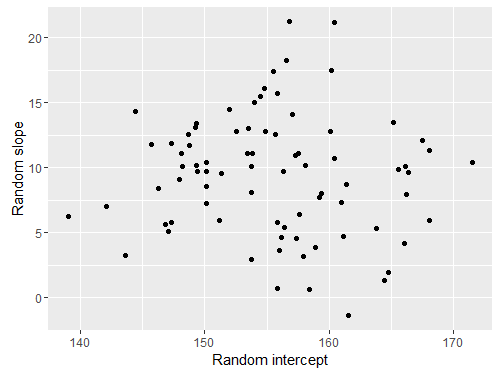
\includegraphics[width=\textwidth]{mainmatter/chapter_5_simulation_study/ds_simple_randplot.png}
       \caption{\label{fig : ds_simple_randplot}Data set 1}
	\end{subfigure}    
	\begin{subfigure}[b]{0.4\textwidth}
		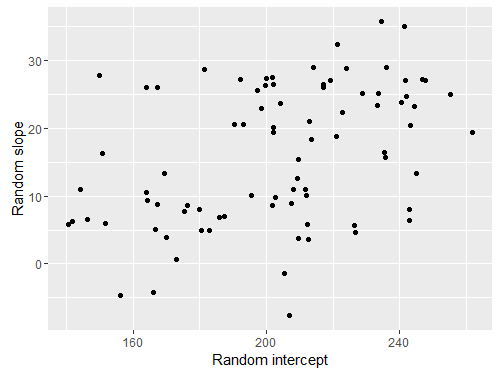
\includegraphics[width=\textwidth]{mainmatter/chapter_5_simulation_study/missing_continuous_covariate_randplot.png}
       \caption{\label{fig : missing_continuous_covariate_randplot} Data set 2: Missing covariate age}
	\end{subfigure}     
\caption{\label{fig : ds_simple_n_3wellsep}Rough estimate $\boldsymbol{\hat{b}}_i$ for random effects}
\end{figure}

\subsubsection{Data set 3: 3 well separated components but less subjects}
\label{subsubsec : ds_3wellsep_3ppg}
This data is similar to Data set 2 in all regards except for the number of subjects. We generated only 36 subjects in total in this data set. A plot of the rough estimates of random effect values for this data set is shown in figure \ref{fig : ds_3wellsep3ppg_randplot}.

\subsubsection{Data set 4: 3 fused components for the mixture of random effects}
\label{subsubsec : ds_3fused_10ppg}
In this data set we simulated the random effects from a mixture distribution which had 3 fused components. For e.g. if one sees the plot of the rough estimates of random effect values for this data set (figure \ref{fig : ds_3fused10ppg_randplot}) then it is not clear if there are more than 2 components.

\begin{figure}[!htb]
\centering
\captionsetup{justification=centering}
\begin{subfigure}[b]{0.4\textwidth}
		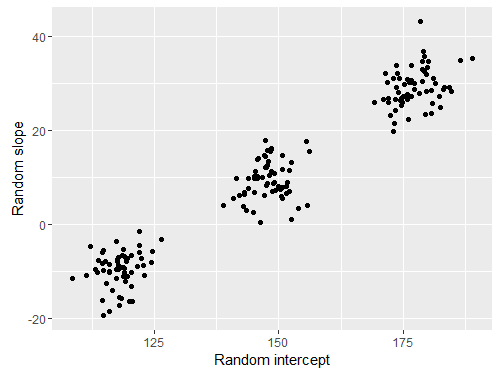
\includegraphics[width=\textwidth]{mainmatter/chapter_5_simulation_study/ds_3wellsep_randplot.png}
        \caption{\label{fig : ds_3wellsep_randplot}Data set 2}
	\end{subfigure}
	\begin{subfigure}[b]{0.4\textwidth}
		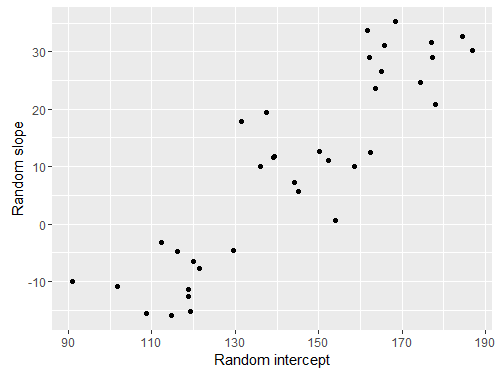
\includegraphics[width=\textwidth]{mainmatter/chapter_5_simulation_study/ds_3wellsep3ppg_randplot.png}
       \caption{\label{fig : ds_3wellsep3ppg_randplot}Data set 3}
	\end{subfigure}    
    
\caption{\label{fig : ds_3comp_3ppgwelsep}Rough estimate $\boldsymbol{\hat{b}}_i$ for random effects}
\end{figure}

\subsubsection{Data set 5: 3 fused components but less subjects}
\label{subsubsec : ds_3fused_3ppg}
This data is similar to Data set 4 in all regards except for the number of subjects. We generated only 36 subjects in total in this data set. A plot of the rough estimates of random effect values for this data set is shown in figure \ref{fig : ds_3fused3ppg_randplot}.

\subsubsection{Data set 6: 5 well separated components}
\label{subsubsec : ds_5wellsep}
In this data set we simulated the random effects from a mixture distribution which had 5 well separated components. However this time we generated unequal number of subjects for every component. The plot of the rough estimates of random effect values for this data set is shown in figure \ref{fig : ds_5wellsep_randplot}.

\begin{figure}[!htb]
\centering
\captionsetup{justification=centering}
\begin{subfigure}[b]{0.4\textwidth}
		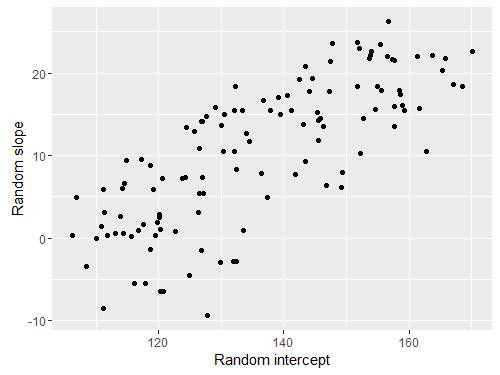
\includegraphics[width=\textwidth]{mainmatter/chapter_5_simulation_study/ds_3fused10ppg_randplot.png}
        \caption{\label{fig : ds_3fused10ppg_randplot}Data set 4}
	\end{subfigure}
	\begin{subfigure}[b]{0.4\textwidth}
		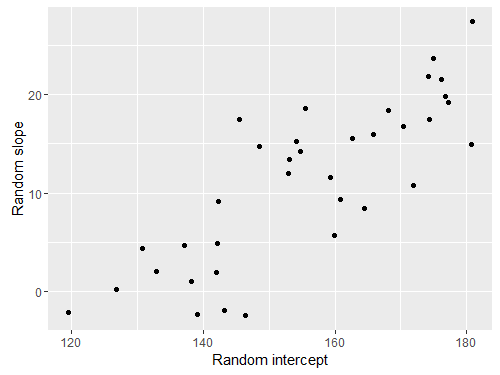
\includegraphics[width=\textwidth]{mainmatter/chapter_5_simulation_study/ds_3fused3ppg_randplot.png}
       \caption{\label{fig : ds_3fused3ppg_randplot}Data set 5}
	\end{subfigure}    
    
\caption{\label{fig : ds_3fused10ppg_3fused3ppg}Rough estimate $\boldsymbol{\hat{b}}_i$ for random effects}
\end{figure}

\subsubsection{Data set 7: 5 fused components}
\label{subsubsec : ds_5fused}
This data is similar to Data set 6 in all regards except that the number of subjects per component are less, and the components are not so well separated. The plot of the rough estimates of random effect values for this data set is shown in figure \ref{fig : ds_5fused_randplot}.

\begin{figure}[!htb]
\centering
\captionsetup{justification=centering}
\begin{subfigure}[b]{0.4\textwidth}
		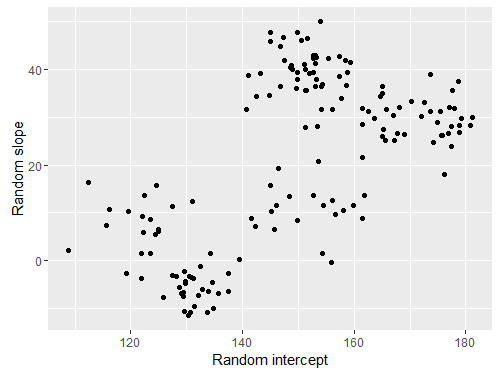
\includegraphics[width=\textwidth]{mainmatter/chapter_5_simulation_study/ds_5wellsep_randplot.png}
        \caption{\label{fig : ds_5wellsep_randplot}Data set 6}
	\end{subfigure}
	\begin{subfigure}[b]{0.4\textwidth}
		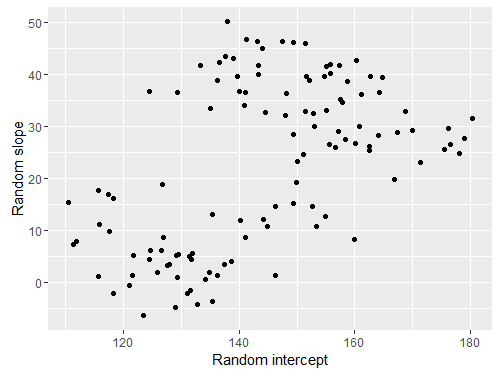
\includegraphics[width=\textwidth]{mainmatter/chapter_5_simulation_study/ds_5fused_randplot.png}
        \caption{\label{fig : ds_5fused_randplot}Data set 7}
	\end{subfigure}
	\caption{Rough estimate $\boldsymbol{\hat{b}}_i$ for random effects.}
	\label{fig : ds_5wellsep_5fused}    
\end{figure}


\subsection{Running MCMC simulations}
We first discuss some of the issues we encountered while doing the MCMC simulations. The first one was label switching across the chains while calculating marginal likelihood using Chib's approximation; i.e. label 1 corresponding to component 1 in one chain and corresponding to some other component in another chain. This gave inconsistent and incorrect estimates for the various calculations we did. Although we dealt with it using the mechanisms given in section \ref{subsec : label_switching_blmm}, mechanisms such as applying an identifiability constraint decreased the speed of simulations drastically. The second issue was high autocorrelation in the chains. We tried various strategies for it. For e.g. using a marginal model was helpful and so was hierarchical centering.\\

However despite these taking these measures we had to employ a thinning of 1 per 100 iterations and in some cases 1 per 200 iterations to make sure the resulting chains were not autocorrelated. Since we lacked computational resources required to run longer chains we had to be content with chains of length 1300 (after thinning). Lastly, we observed that in models where mixture of random effects were fitted with more components than needed, there was very high autocorrelation in the chain which could not be reduced despite high thinning. The convergence tests for such chains showed that the chains did not converge for the parameters of some (this varied from model to model) of the component densities. The parameters corresponding to fixed effects converged in such chains though. Since some of the chains were not converged, it made little sense to compare DIC and marginal likelihood based on such models with models for which the chains converged. Thus we have not presented DIC and marginal likelihood for overfitted models.

\subsection{Deviance information criteria}
\label{subsec : dic_simulation_results}
The Deviance information criteria results are based on a single chain and have been rounded to the nearest integer. Table \ref{table : ds_simple_dic} shows the values of the various deviance information criteria (section \ref{sec : dic}) applied to data set 1. Since data set 1 has no mixture of random effects, models with 2 or more components overfitted the data. As we mentioned earlier that the chains did not converge for some of the parameters in the models with more components than needed, and hence DIC is not presented for them.\\

\begin{table}[!htb]
\centering
\captionsetup{justification=centering}
\caption{DIC and $\text{p}_\text{D}$ for data set 1. True number of components = 1}
\label{table : ds_simple_dic} 
\begin{tabular}{@{}rrrrrrr@{}}
\toprule
\# Comp Fitted & $\text{DIC}_1$ & $\text{DIC}_2$  & $\text{DIC}_3$  & $\text{DIC}_4$  & $\text{DIC}_5$  & $\text{DIC}_6$  \\ \midrule
1      & 4143 & 4144 & 4143 & 5160 & 4402 & 3483 \\
\bottomrule
\end{tabular}

\begin{tabular}{@{}rrrrrrr@{}}
\toprule
\# Comp Fitted & ${\text{p}_\text{D}}_1$ & ${\text{p}_\text{D}}_2$ & ${\text{p}_\text{D}}_3$ & ${\text{p}_\text{D}}_4$ & ${\text{p}_\text{D}}_5$ & ${\text{p}_\text{D}}_6$ \\ \midrule
1      & 9    & 9    & 9    & 903  & 145  & 125  \\
\bottomrule
\end{tabular}
\end{table}

Table \ref{table : ds_3wellsep_dic} shows the values of various DIC we obtained for data set 2. One of the observations from these results is that $\text{DIC}_4$ is the most discerning among all of the DIC's. $\text{DIC}_6$ prefers model with no mixture over models with 2 or 3 components, and hence it is not reliable. The rest of the DIC select the model with the right number of components.\\

\begin{table}[!htb]
\centering
\captionsetup{justification=centering}
\caption{DIC and $\text{p}_\text{D}$ for data set 2. True number of components = 3}
\label{table : ds_3wellsep_dic} 
\begin{tabular}{@{}rrrrrrr@{}}
\toprule
\# Comp Fitted & $\text{DIC}_1$ & $\text{DIC}_2$  & $\text{DIC}_3$  & $\text{DIC}_4$  & $\text{DIC}_5$  & $\text{DIC}_6$  \\ \midrule
1 & 9966 & 9959 & 9965 & 12921 & 10531 & 7855 \\
2 & 9865 & 9849 & 9864 & 12498 & 10458 & 7860 \\
3 & 9664 & 9665 & 9663 & 11847 & 10244 & 7870 \\
\bottomrule
\end{tabular}

\begin{tabular}{@{}rrrrrrr@{}}
\toprule
\# Comp Fitted & ${\text{p}_\text{D}}_1$ & ${\text{p}_\text{D}}_2$ & ${\text{p}_\text{D}}_3$ & ${\text{p}_\text{D}}_4$ & ${\text{p}_\text{D}}_5$ & ${\text{p}_\text{D}}_6$ \\ \midrule
1 & 9 & 2 & 8 & 2670 & 279 & 269 \\
2 & 15 & -1 & 14 & 2344 & 304 & 272 \\
3 & 21 & 21 & 20 & 1933 & 331 & 282 \\
\bottomrule
\end{tabular}
\end{table}

Table \ref{table : ds_3wellsep_3ppg_dic} shows the values of the various DIC applied to the data set 3. Firstly we can see that $\text{DIC}_6$ prefers model with 2 components over a model with 3 components, which is an incorrect choice of the number of the components in mixture. $\text{DIC}_5$ exhibits the same problem and hence is not reliable. The rest of the DIC select the model with the right number of components. However, once again it is $\text{DIC}_4$ which discerns the most among the various models. The magnitudes of all of the DIC for this data set were less in comparison to DIC for data set 2 because the sample size for this data set was only 36 subjects compared to 180 subjects in the former.\\

\begin{table}[!htb]
\centering
\captionsetup{justification=centering}
\caption{DIC and $\text{p}_\text{D}$ for data set 3. True number of components = 3}
\label{table : ds_3wellsep_3ppg_dic}
\begin{tabular}{@{}rrrrrrr@{}}
\toprule
\# Comp Fitted & $\text{DIC}_1$ & $\text{DIC}_2$  & $\text{DIC}_3$  & $\text{DIC}_4$  & $\text{DIC}_5$  & $\text{DIC}_6$  \\ \midrule
1 & 2013 & 2012 & 2012 & 2611 & 2118 & 1570 \\
2 & 1989 & 1949 & 1987 & 2497 & 2013 & 1562 \\
3 & 1942 & 1942 & 1940 & 2339 & 2039 & 1571 \\
\bottomrule
\end{tabular}

\begin{tabular}{@{}rrrrrrr@{}}
\toprule
\# Comp Fitted & ${\text{p}_\text{D}}_1$ & ${\text{p}_\text{D}}_2$ & ${\text{p}_\text{D}}_3$ & ${\text{p}_\text{D}}_4$ & ${\text{p}_\text{D}}_5$ & ${\text{p}_\text{D}}_6$ \\ \midrule
1 & 8 & 7 & 7 & 545 & 52 & 45 \\
2 & 14 & -26 & 12 & 465 & -20 & 35 \\
3 & 17 & 17 & 15 & 370 & 70 & 46 \\
\bottomrule
\end{tabular}
\end{table}

Table \ref{table : ds_3fused_10ppg_dic} shows the results of applying various DIC to data set 4. So far we have observed that $\text{DIC}_1$ to $\text{DIC}_4$ can be used to detect the right number of components. From the table of DIC it is clear that $\text{DIC}_1$ to $\text{DIC}_4$ can still be used to select the right number of components, however $\text{DIC}_6$ chose model 1 over model with higher number of components. $\text{DIC}_5$ has almost the same value for Model with no mixture and model with 3 components in the mixture. Thus once again both $\text{DIC}_5$ and  $\text{DIC}_6$ cannot be considered reliable. To further validate the results, we decided to decrease the number of subjects to 36.\\
 
\begin{table}[!htb]
\centering
\captionsetup{justification=centering}
\caption{DIC and $\text{p}_\text{D}$ for data set 4. True number of components = 3}
\label{table : ds_3fused_10ppg_dic}
\begin{tabular}{@{}rrrrrrr@{}}
\toprule
\# Comp Fitted & $\text{DIC}_1$ & $\text{DIC}_2$  & $\text{DIC}_3$  & $\text{DIC}_4$  & $\text{DIC}_5$  & $\text{DIC}_6$  \\ \midrule
1 & 6568 & 6566 & 6566 & 8454 & 6899 & 5197 \\
2 & 6531 & 6523 & 6530 & 8263 & 6946 & 5253 \\
3 & 6497 & 6492 & 6497 & 8017 & 6898 & 5263 \\
\bottomrule
\end{tabular}

\begin{tabular}{@{}rrrrrrr@{}}
\toprule
\# Comp Fitted & ${\text{p}_\text{D}}_1$ & ${\text{p}_\text{D}}_2$ & ${\text{p}_\text{D}}_3$ & ${\text{p}_\text{D}}_4$ & ${\text{p}_\text{D}}_5$ & ${\text{p}_\text{D}}_6$ \\ \midrule
1 & 9 & 8 & 8 & 1694 & 139 & 127 \\
2 & 14 & 7 & 13 & 1527 & 210 & 182 \\
3 & 20 & 14 & 19 & 1341 & 222 & 187 \\
\bottomrule
\end{tabular}
\end{table}

Table \ref{table : ds_3fused_3ppg_dic} shows the results of calculating DIC for models applied to data set 5. The peculiarity of this data set was that the number of subjects were less and the components were fused. Thus we observed that some of the components remained empty even when we fitted the right number of components, and further the chains did not converge. As we discussed in section \ref{subsec : choice_priors} one could use a Dirichlet prior with slightly bigger hyperparameters to avoid empty components, although at the risk of becoming too informative. For the model with 2 components, we tried various hyperparameter values between 0 and 3 and found that increasing the hyperparameter beyond 2.5 was not necessary as the chains were converged with a $\text{Dir}(2.5, 2.5, ..., 2.5)$ prior on weight distribution. However for a model with 3 components we had to choose a $\text{Dir}(5, 5, ..., 5)$ prior to obtain chains which were converged and had posterior component density parameter values near the actual ones. The most interesting aspect of the results was that for 4 components we could not get converged chains even when we used $\text{Dir}(20, 20, ..., 20)$ prior. We also modeled the data using smaller values for Dirichlet prior hyperparameters; for e.g. $\text{Dir}(0.1, 0.1, ..., 0.1)$ and $\text{Dir}(0.6, 0.6, ..., 0.6)$ prior were tested. However both of these priors performed as worse as the $\text{Dir}(1, 1, ..., 1)$ prior for the current data set. All other DIC's other than $\text{DIC}_5$ and $\text{DIC}_6$ select the right number of components for this data set. $\text{DIC}_4$ is once again the most discerning DIC.\\

\begin{table}[!htb]
\centering
\captionsetup{justification=centering}
\caption{DIC and $\text{p}_\text{D}$ for data set 5. True number of components = 3}
\label{table : ds_3fused_3ppg_dic}
\begin{tabular}{@{}rrrrrrr@{}}
\toprule
\# Comp Fitted & $\text{DIC}_1$ & $\text{DIC}_2$  & $\text{DIC}_3$  & $\text{DIC}_4$  & $\text{DIC}_5$  & $\text{DIC}_6$  \\ \midrule
1 & 1944 & 1943 & 1943 & 2500 & 1879 & 1364 \\
2 & 1934 & 1936 & 1936 & 2438 & 2042 & 1526 \\
3 & 1921 & 1920 & 1922 & 2350 & 2023 & 1537\\
\bottomrule
\end{tabular}

\begin{tabular}{@{}rrrrrrr@{}}
\toprule
\# Comp Fitted & ${\text{p}_\text{D}}_1$ & ${\text{p}_\text{D}}_2$ & ${\text{p}_\text{D}}_3$ & ${\text{p}_\text{D}}_4$ & ${\text{p}_\text{D}}_5$ & ${\text{p}_\text{D}}_6$ \\ \midrule
1 & 9 & 7 & 7 & 510 & -110 & -119 \\
2 & 11 & 14 & 13 & 460 & 63 & 43 \\
3 & 16 & 14 & 17 & 396 & 69 & 53 \\
\bottomrule
\end{tabular}
\end{table}

Table \ref{table : ds_5wellsep_dic} shows the results of applying DIC to the various models fitted for data set 6. $\text{DIC}_5$ and $\text{DIC}_6$ give smallest DIC for underfitted models once again. The rest of the DIC's select the model with the right number of components.\\

\begin{table}[!htb]
\centering
\captionsetup{justification=centering}
\caption{DIC and $\text{p}_\text{D}$ for data set 6. True number of components = 5}
\label{table : ds_5wellsep_dic}
\begin{tabular}{@{}rrrrrrr@{}}
\toprule
\# Comp Fitted & $\text{DIC}_1$ & $\text{DIC}_2$  & $\text{DIC}_3$  & $\text{DIC}_4$  & $\text{DIC}_5$  & $\text{DIC}_6$  \\ \midrule
1 & 8982 & 8981 & 8980 & 11847 & 9251 & 6655 \\
2 & 8829 & 8827 & 8827 & 11327 & 9293 & 6838 \\
3 & 8745 & 8742 & 8744 & 11036 & 9251 & 6895 \\
4 & 8669 & 8672 & 8677 & 10737 & 9208 & 6925 \\
5 & 8649 & 8643 & 8648 & 10601 & 9165 & 6909 \\
\bottomrule
\end{tabular}

\begin{tabular}{@{}rrrrrrr@{}}
\toprule
\# Comp Fitted & ${\text{p}_\text{D}}_1$ & ${\text{p}_\text{D}}_2$ & ${\text{p}_\text{D}}_3$ & ${\text{p}_\text{D}}_4$ & ${\text{p}_\text{D}}_5$ & ${\text{p}_\text{D}}_6$ \\ \midrule
1 & 9 & 9 & 7 & 2591 & -5 & -14 \\
2 & 14 & 13 & 12 & 2224 & 190 & 169 \\
3 & 20 & 16 & 19 & 2035 & 250 & 223 \\
4 & 19 & 23 & 27 & 1824 & 296 & 251 \\
5 & 31 & 26 & 30 & 1725 & 289 & 232 \\
\bottomrule
\end{tabular}
\end{table}

\begin{table}[!htb]
\centering
\captionsetup{justification=centering}
\caption{DIC and $\text{p}_\text{D}$ for data set 7. True number of components = 5}
\label{table : ds_5fused_dic}
\begin{tabular}{@{}rrrrrrr@{}}
\toprule
\# Comp Fitted & $\text{DIC}_1$ & $\text{DIC}_2$  & $\text{DIC}_3$  & $\text{DIC}_4$  & $\text{DIC}_5$  & $\text{DIC}_6$  \\ \midrule
1 & 6708 & 6707 & 6706 & 8819 & 6977 & 5071 \\
2 & 6606 & 6605 & 6604 & 8443 & 6946 & 5135 \\
3 & 6539 & 6538 & 6537 & 8178 & 6944 & 5204 \\
4 & 6506 & 6514 & 6521 & 8078 & 6915 & 5196 \\
5 & 6505 & 6500 & 6508 & 7984 & 6896 & 5202 \\
\bottomrule
\end{tabular}

\begin{tabular}{@{}rrrrrrr@{}}
\toprule
\# Comp Fitted & ${\text{p}_\text{D}}_1$ & ${\text{p}_\text{D}}_2$ & ${\text{p}_\text{D}}_3$ & ${\text{p}_\text{D}}_4$ & ${\text{p}_\text{D}}_5$ & ${\text{p}_\text{D}}_6$ \\ \midrule
1 & 9 & 8 & 7 & 1903 & 61 & 53 \\
2 & 15 & 14 & 13 & 1636 & 139 & 120 \\
3 & 21 & 20 & 19 & 1456 & 221 & 185 \\
4 & 12 & 20 & 26 & 1381 & 218 & 176 \\
5 & 26 & 22 & 29 & 1308 & 220 & 182 \\
\bottomrule
\end{tabular}
\end{table}

Table \ref{table : ds_5fused_dic} shows the results of applying DIC to the various models fitted for data set 7. Based on figure \ref{fig : ds_5fused_randplot} it is difficult to identify more than 3 components in this mixture. However once again $\text{DIC}_4$ appeared to be identifying the right number of components correctly. $\text{DIC}_2$ and $\text{DIC}_3$ do not seem to discern much among the various models, which as we saw earlier, happens when the components are fused. Interestingly $\text{DIC}_1$ selects the right model only by virtue of a difference of DIC value of 1 between model with 4 components and 5 components.\\

It is important to note that when components were fused, then even with a very large number of MCMC iterations we observed a variation of 10 to 20 in the same DIC across chains. Thus, although $\text{DIC}_3$ preferred model 5 over model 4 by a DIC difference of 13, it is highly plausible to obtain a difference of -7; i.e. Model 4 having a lower $\text{DIC}_3$ than model 5. In such a case if the classical rule of thumb of DIC difference of 5 to 10 is used to select the models then an incorrect model might get selected.

\subsection{Marginal likelihood}
\label{subsec : marginal_likelihood_simulation}
To calculate marginal likelihood for the various models we implemented Chib's approximation described in section \ref{sec : marginal_likelihood}. Table \ref{table : marginal_likelihood_results} shows the results of $\log{\hat{m}(\boldsymbol{y})}$ for the various models we fitted to data set 1 to data set 7. One can see that even among the well converged models there is no obvious pattern visible in these results to conclude the efficacy of marginal likelihood in selection of a model. For e.g. in case of data set 6 there were 5 well separated components in the mixture distribution of random effects. When we fitted 1 to 5 components for this data set we obtained MCMC chains with good convergence. However in table \ref{table : marginal_likelihood_results} we can see that marginal likelihood prefers fitting 4 components over 5 components. For data set 3 where we had 3 well separated components but only 36 subjects in total, we can observe that marginal likelihood incorrectly prefers model with 1 components and not model with 3 components. Thus marginal likelihood using Chib's approximation does not seem to be a very reliable method to choose the correct Bayesian heterogeneity model.

\begin{table}[!htb]
\centering
\captionsetup{justification=centering}
\caption{$\log{\hat{m}(\boldsymbol{y})}$ for data set 1}
\label{table : marginal_likelihood_results} 
\begin{tabular}{lrrrrr}
\toprule
Fitted & 1 Comp & 2 Comp & 3 Comp & 4 Comp & 5 Comp \\\midrule
Data set 1 & -2120 & & & & \\
Data set 2 & -5019 & -4989 & -4937 & & \\
Data set 3 & -1038 & -1044 & -1042 & & \\
Data set 4 & -3317 & -3318 & -3322 & & \\
Data set 5 & -1001 & -986 & -993 & &  \\
Data set 6 & -4545 & -4492 & -4477 & -4467 & -4473\\
Data set 7 & -3397 & -3379 & -3373 & -3380 & -2749\\ \bottomrule
\end{tabular}
\end{table}

\subsection{Posterior predictive check (PPC)}
\label{subsec : ppc_simulation}
We implemented the PPC outlined in section \ref{sec : ppc} and found that it worked quite well irrespective of the size of the data set or how well separated the components were. Secondly, since the PPC we used was designed to detect non identifiability due to empty components it worked well for models which were overfitting and thus had empty components. It is important to note that for such models, the convergence diagnostics did not show any evidence against convergence of chains for fixed effect coefficients. It were only some of the component densities whose parameters which did not converge, which as we mentioned earlier, varied from model to model.\\

\begin{figure}[!htb]
\centering
\captionsetup{justification=centering}
\begin{subfigure}[b]{0.4\textwidth}
		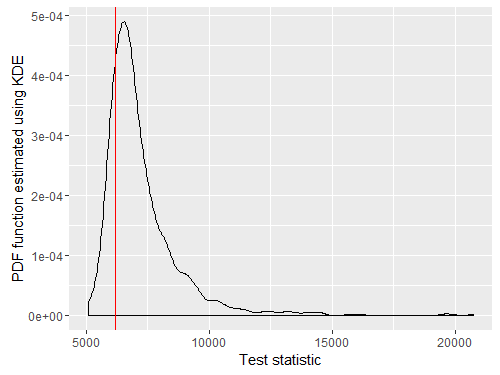
\includegraphics[width=\textwidth]{mainmatter/chapter_5_simulation_study/ppc_5wellsep8comp.png}
        \caption{\label{fig : ppc_5wellsep8comp} \# components fitted = 8}
	\end{subfigure}
	\begin{subfigure}[b]{0.4\textwidth}
		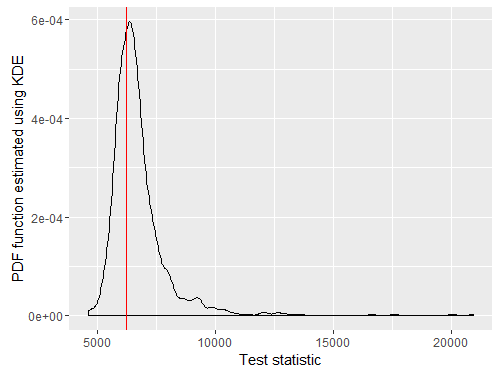
\includegraphics[width=\textwidth]{mainmatter/chapter_5_simulation_study/ppc_5wellsep7comp.png}
          \caption{\label{fig : ppc_5wellsep7comp}\# components fitted = 7}
	\end{subfigure}
	\begin{subfigure}[b]{0.4\textwidth}
		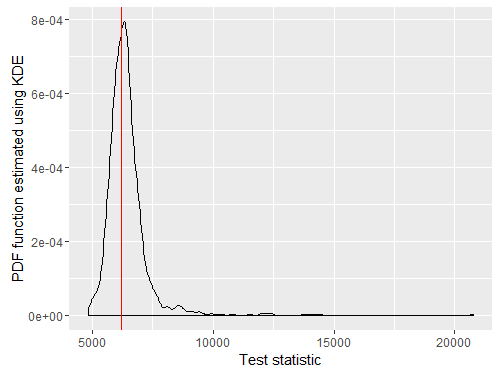
\includegraphics[width=\textwidth]{mainmatter/chapter_5_simulation_study/ppc_5wellsep6comp.png}
          \caption{\label{fig : ppc_5wellsep6comp}\# components fitted = 6}
	\end{subfigure}
	
	\caption{Density function of $T(\boldsymbol{\tilde{r}})$ for overfitted models applied to data set 6. The red line shows the value of the test statistic $T(\boldsymbol{r})$ based on the observed data.}
	\label{fig : ppc_5wellsepcomp_overfitted}    
\end{figure}

\begin{figure}[!htb]
\centering
\captionsetup{justification=centering}
	\begin{subfigure}[b]{0.4\textwidth}
		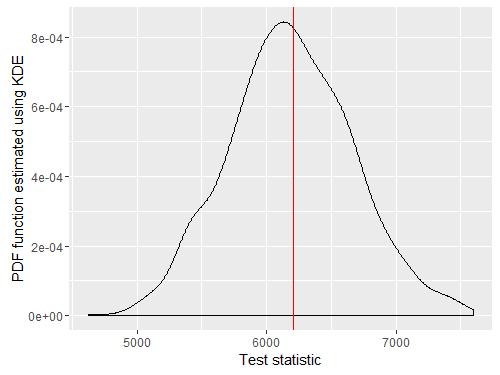
\includegraphics[width=\textwidth]{mainmatter/chapter_5_simulation_study/ppc_5wellsep5comp.png}
          \caption{\label{fig : ppc_5wellsep5comp}\# components fitted = 5}
	\end{subfigure}
	\begin{subfigure}[b]{0.4\textwidth}
		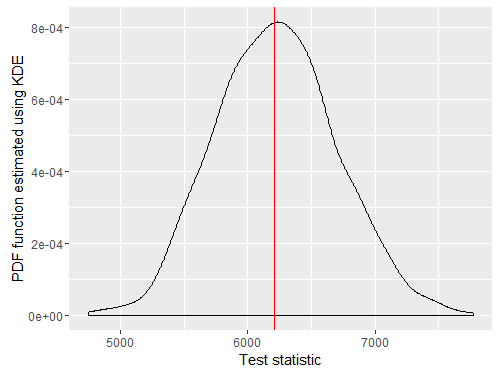
\includegraphics[width=\textwidth]{mainmatter/chapter_5_simulation_study/ppc_5wellsep4comp.png}
          \caption{\label{fig : ppc_5wellsep4comp}\# components fitted = 4}
	\end{subfigure}
	\begin{subfigure}[b]{0.4\textwidth}
		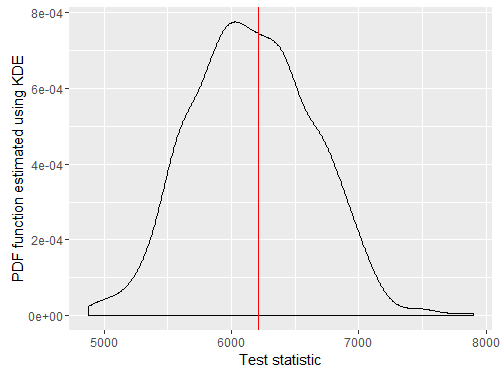
\includegraphics[width=\textwidth]{mainmatter/chapter_5_simulation_study/ppc_5wellsep3comp.png}
          \caption{\label{fig : ppc_5wellsep3comp}\# components fitted = 3}
	\end{subfigure}
	\begin{subfigure}[b]{0.4\textwidth}
		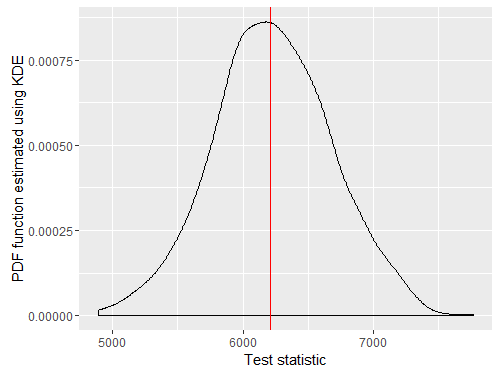
\includegraphics[width=\textwidth]{mainmatter/chapter_5_simulation_study/ppc_5wellsep2comp.png}
          \caption{\label{fig : ppc_5wellsep2comp}\# components fitted = 2}
	\end{subfigure}
	\begin{subfigure}[b]{0.4\textwidth}
		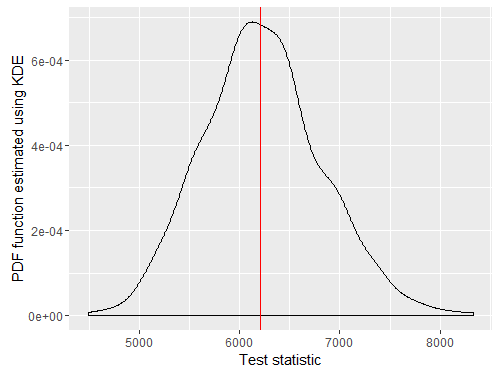
\includegraphics[width=\textwidth]{mainmatter/chapter_5_simulation_study/ppc_5wellsep1comp.png}
          \caption{\label{fig : ppc_5wellsep1comp}\# components fitted = 1}
	\end{subfigure}
	\caption{Density function of $T(\boldsymbol{\tilde{r}})$ for under/rightly fitted models applied to data set 6. The red line shows the value of the test statistic $T(\boldsymbol{r})$ based on the observed data.}
	\label{fig : ppc_5wellsepcomp_underfitted}    
\end{figure}

We found the results of PPC to be very consistent across the various data sets and so we discuss only the results of fitting various number of components to data set 6. Figure \ref{fig : ppc_5wellsepcomp_overfitted} and figure \ref{fig : ppc_5wellsepcomp_underfitted} show the distribution of the test statistic in equation \ref{eq : ppc_test_statistic} for the various models we fitted to data set 6. It can be seen that the distribution is positively skewed whenever overfitting is present, which can be attributed to sampling from empty components as we discussed in section \ref{subsec : ppc_bhtge}. On the other hand the distribution of the test statistic is more or less the same in cases of underfitting.\\

\begin{table}[!htb]
\centering
\captionsetup{justification=centering}
\caption{PPP values for the various models fitted to data set 6.}
\label{table : ppp_value_5welsepcomp}
\begin{tabular}{@{}rrrrrrrrr@{}}
\toprule
\# Components fitted & 1 & 2 & 3 & 4 & 5 & 6 & 7 & 8 \\ \midrule
PPP Value & 0.500 & 0.500 & 0.492 & 0.500 & 0.500 & 0.581 & 0.674 & 0.775 \\ \bottomrule
\end{tabular}
\end{table}

We also calculated posterior predictive p-values for the various number of components we fitted to data set and they are presented in table \ref{table : ppp_value_5welsepcomp}. As one can see the PPP values are equal (0.5) for all the underfitted models. Based on the graphical PPC and these PPP values, it was not possible to choose a model among the correctly fitted and underfitted one. On the other hand for models with overfitted components, the PPP values increase as overfitting increases.\\

We observed a more severe impact of overfitting when we used independent inverse gamma priors for the variance components of $G_k$ and uniform prior $U(-1,1)$ for correlation. To show the resulting distribution of the test statistic, we had to log transform it because otherwise the values were too large to be plotted in a single graph. For data set 2 we overfitted the mixture of random effects by using 4 components in the mixture. As shown in Figure \ref{fig : ppc_3wellsep4comp_indp_gammaprior} the test statistic is inflated by a large margin, which was also discussed in section \ref{sec : ppc}. Interestingly when we fitted the right number of components the test statistic was not inflated, but the model was not fitting well to the data as shown in Figure \ref{fig : ppc_3wellsep3comp_indp_gammaprior}. The PPP-value we observed was 1. To diagnose this problem we checked the posteriors for variance covariance matrices and found them to be underestimating the sample data's variance covariance of the random effects. This indicated that the test statistic can be used to detect an overall bad model fit even when the right number of components are fitted to the mixture distribution of random effects.\\

\begin{figure}[!htb]
	\centering
	\captionsetup{justification=centering}
	\begin{subfigure}[b]{0.4\textwidth}
		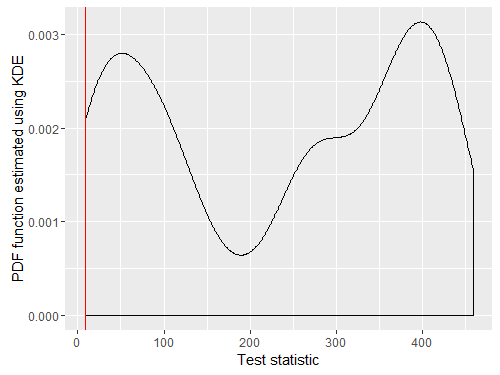
\includegraphics[width=\textwidth]{mainmatter/chapter_5_simulation_study/indpGammaPrior_ppc_3wellsep4comp.png}
        \caption{\label{fig : ppc_3wellsep4comp_indp_gammaprior}4 components fitted for data set 2. log scale is used.}
	\end{subfigure}
	\begin{subfigure}[b]{0.4\textwidth}
		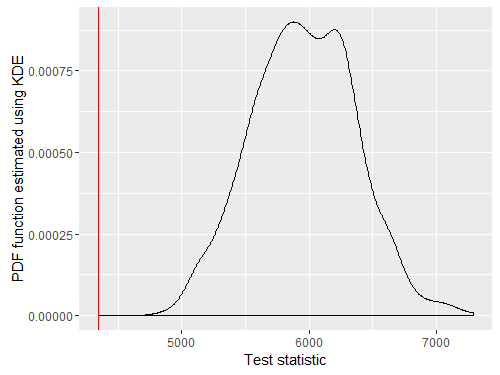
\includegraphics[width=\textwidth]{mainmatter/chapter_5_simulation_study/indpGammaPrior_ppc_3wellsep3comp.png}
        \caption{\label{fig : ppc_3wellsep3comp_indp_gammaprior}3 components fitted for data set 2}
	\end{subfigure}
	\caption{PDF function of $T(\boldsymbol{\tilde{r}})$ estimated using KDE. The red line shows the value of the test statistic $T(\boldsymbol{r})$ based on the observed data. Independent inverse gamma priors for variance of random effects and uniform prior for correlation is used.}
	\label{fig : ppc_3wellsepcomp_indp_gammaprior}
\end{figure}
% !TEX root =  ../../thesis.tex

\chapter{Analysis of blood donor data set}
\label{ch : blood_donor}
 
 In this chapter we present the analysis of the blood donor data set \citep{nasserinejad_prevalence_2015} using the Bayesian heterogeneity model. The data set consists of 1595 male blood donors who donated blood multiple times over a period of many years. On each visit to the donation center, the following information was noted: Season in which blood was donated (Cold/Hot), Volume of blood donated (ml), age at the time of donation (years), a binary indicator Donate (yes/no) specifying if the donor was allowed to donate the blood, Hemoglobin (Hb) of the patient at the time of donation, and the date of visit. Other variables derived from date of visit such as time since previous donation (TSPD), time since previous visit (TSPV) were also present in the data set. \citet{nasserinejad_predicting_2013,nasserinejad_prevalence_2015,nasserinejad_prediction_2016} have analyzed this data set extensively using transition models, mixed models, growth mixture models and latent class mixed effects transition models. The analysis was used to predict the Hb level of donors so that they are invited for donation at an optimal time, i.e. when their Hb levels are not too low because of the previous donations and other factors.\\

 For the purpose of this thesis we did not use the entire data set of 1595 patients as Bayesian computation for heterogeneity model using the entire data set required large amount of computational resources. Instead we used a simple random sample of the data consisting of 250 subjects.

\section{Motivation for analysis with Bayesian heterogeneity model}
 In the analysis using growth mixture models \citet{nasserinejad_prevalence_2015} found 4 different underlying subpopulations in the data set. Firstly, those which had a relatively stable Hb level over donations. Secondly, those which had a higher baseline Hb level than those in category 1 and also showed a slow decline of Hb level over donations. Thirdly, those which showed a moderately sharp decline in Hb level over donations, and lastly those which showed a steep decline in Hb levels despite beginning at high initial Hb levels. Because of the presence of different subpopulations, a single methodology to decide the time of next blood donation for subjects from all subpopulations may not be effective. The aim of applying the Bayesian heterogeneity model to this dataset was to provide an alternative modeling framework for such data sets.

\section{Frequentist analysis}
\label{sec : frequentist_blood_donor}
We began with a frequentist analysis of the blood donor data set to select the right mean structure for our models ahead. This was necessary because omitting a required covariate in the mean structure could lead to incorrect estimates of the covariance matrix. Secondly, a frequentist analysis provided us good starting values for the various parameters in our model. Thirdly we also wanted check if the Bayesian analysis results were consistent with the frequentist analysis results. For the random effects structure we considered a model with both random intercept and random slope. For the choice of random slope we selected the variable 'number of donations in last 2 years' because that was deemed as a suitable variable for random slope by \citet{nasserinejad_prevalence_2015}. For selecting the mean structure we did F-tests and likelihood ratio tests based on ML. We found the following mean structure to be suitable.

\begin{equation}
\label{eq : blood_donor_model}
\begin{split}
\boldsymbol{y}_{ij} = \beta_0 + \beta_1*\text{Age}_{ij} + \beta_2*\text{Season}_{ij} + \beta_3*\text{Donate}_{ij} + \beta_4*\text{TSPD}_{ij}\\
+ \beta_4*\text{\#donationLast2Years}_{ij} + \beta_5*\text{\#donationLast2Years}_{ij}*\text{TSPD}_{ij}\\
+ \beta_6*\text{\#donationLast2Years}_{ij}*\text{Donate}_{ij} + \beta_7*\text{\#donationLast2Years}_{ij}^2\\
+ b_0 + b_1 * \text{\#donationLast2Years}_{ij} + \varepsilon_{ij}
\end{split}
\end{equation}

where, Age and TSPD have been standardized to have mean 0 and variance 1, $\text{\#donationLast2Years}_{ij}$ have been downscaled by a factor of 100 so that the random slope variance scale is upscaled. Similarly the intercept we used was 0.1, thus upscaling the random intercept variance. It is important to note that this model assumes a single multivariate normal distribution for the distribution of random effects. Table \ref{table : frequentist_fixed effects} shows the parameter estimates for this model. 

\begin{table}[!htb]
\centering
\captionsetup{justification=centering}
\caption{Frequentist fixed effect estimates and random variance estimates for model \ref{eq : blood_donor_model}. REML was used for obtaining these parameter estimates.}
\label{table : frequentist_fixed effects}
\begin{tabular}{@{}lrr@{}}
\toprule
Fixed Effects ($\beta$) & Mean & Standard Error \\ \midrule
intercept & 94.121 & 0.429 \\
Age & -0.086 & 0.026 \\
\#donationLast2Years & -7.265 & 1.555 \\
TSPD & -0.036 & 0.015 \\
Season (Hot) & -0.080 & 0.016 \\
Donate (TRUE) & 0.155 & 0.037 \\
\#donationLast2Years * TSPD & 0.020 & 0.006 \\
\#donationLast2Years * Donate & 4.689 & 0.995 \\
$\text{\#donationLast2Years}^2$ & -52.796 & 15.237 \\ \bottomrule
\end{tabular}

\begin{tabular}{@{}lr@{}}
\toprule
Covariance Parameters & Estimate \\ \midrule
$\sigma^2_\text{Intercept}$ & 19.971 \\
$\sigma_\text{Intercept, Slope}$ & -14.266 \\
$\sigma^2_\text{Slope}$ & 40.183 \\
$\sigma^2$ & 0.201 \\ \bottomrule
\end{tabular}
\end{table}

\section{Bayesian analysis}
\label{sec : blood_donor_bayesian_analysis}
We next extended the model in equation \ref{eq : blood_donor_model} for fitting the Bayesian version of the Heterogeneity model proposed by \citet{verbeke_linear_1996}. Since the random component in the Bayesian heterogeneity model follows a mixture distribution we fitted mixtures of 1 to 5 components. We removed the intercept and the fixed effect of number of donations in last 2 years from the model to impose hierarchical centering on the random effects. The next step we took for model fitting was generating a plot of random part of the model using the approach mentioned in section \ref{subsec : ds_description}. The corresponding plot in figure \ref{fig : rough_idea_blood_donor} indicates that there could be perhaps 1 component, or if there are more components then the components are not well separated. We saw in the case of data set 5 (figure \ref{fig : ds_3fused3ppg_randplot}) which also had fused components, that we required a slightly higher value for the parameters of the Dirichlet prior for weight distribution. Thus we tested $\text{Dir}(1, 1,...1)$, $\text{Dir}(2, 2,...2)$ and $\text{Dir}(3, 3,...3)$ for the blood donor data set. From the various simulations we ran we found that $\text{Dir}(2, 2,...2)$ prior gave the same results as Dirichlet priors with slightly higher values of the hyperparameters and so we stuck with it. As for the length of MCMC chains, we ran 500,000 iterations with a thinning of 150 and a burn in of 100,000 iterations.\\

\begin{figure}
	\centering
	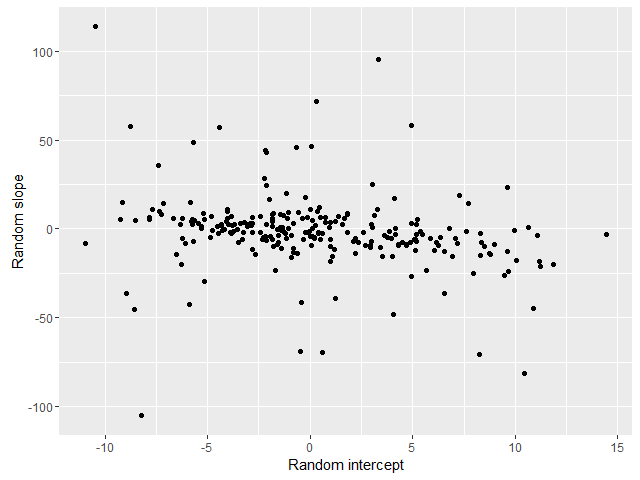
\includegraphics[scale=0.5]{mainmatter/chapter_6_blood_donor/rough_estimate_random_effects.png}
	\caption{Rough estimate $\tilde{\boldsymbol{b}_i}$ for random effects}
	\label{fig : rough_idea_blood_donor}
\end{figure}

The first model we fitted was without any mixture of random effects. The parameter estimates we obtained from this model are shown in table \ref{table : bayesian fixed effects}. It is quite clear from these results that the parameter estimates Bayesian analysis are almost the same as the parameter estimates from frequentist analysis.

\begin{table}[!htb]
\centering
\captionsetup{justification=centering}
\caption{Bayesian fixed effect estimates and random effect estimates for model \ref{eq : blood_donor_model}. The intercept and \#donationLast2Years have been removed for hierarchical centering.}
\label{table : bayesian fixed effects}
\begin{tabular}{@{}lrrr@{}}
\toprule
Fixed Effects ($\beta$) & Mean & Median & 95\% HPDI \\ \midrule
Age & -0.086 & -0.086 & -0.135, -0.034\\
TSPD & -0.037 & -0.037 & -0.068, -0.009 \\
Season (Hot) & -0.080 & -0.080 & -0.109, -0.048\\
Donate (TRUE) & 0.157 & 0.157 & 0.083, 0.232 \\
\#donationLast2Years * TSPD & 0.020 & 0.020 & 0.009, 0.031  \\
\#donationLast2Years * Donate & 4.694 & 4.715 & 2.492, 6.492 \\
$\text{\#donationLast2Years}^2$ & -50.247 & -50.449 & -77.843, -21.436 \\ \bottomrule
\end{tabular}

\begin{tabular}{@{}lrrr@{}}
\toprule
Covariance Parameters & Mean & Median & 95\% HPDI \\ \midrule
$b_{\text{Intercept}}^C$& 94.130 & 94.142 & 93.303, 94.954\\
$b_{\text{slope}}^C$ & -7.504 & -7.531 & -10.639, -4.531\\
$\sigma^2_\text{Intercept}$ & 20.098 & 19.883 & 15.784, 24.559\\
$\sigma_\text{Intercept, Slope}$ & -13.989 & -13.771 & -20.879, -7.903\\
$\sigma^2_\text{Slope}$ & 39.396 & 39.061 & 27.895, 53.443\\
$\sigma^2$ & 0.201 & 0.201 & 0.191, 0.213\\ \bottomrule
\end{tabular}
\end{table}

Next we fitted models with 2 to 5 components in the mixture of random effects. In the case of fitting two components to the mixture we applied identifiability constraints on the weights, i.e. $\eta_1 < \eta_2$. Without these constraints we observed label switching and thus the posteriors were bimodal. For 3 or more components however identifiability constraints were not useful. For e.g. in the case of fitting 3 components we observed convergence only in some chains when we increased the hyperparameters for the Dirichlet prior (prior for $\boldsymbol{\eta}$) to 13. Since the prior was not informative we discarded the corresponding results.\\

Nevertheless for each of the resulting MCMC chains we calculated the various definitions of DIC given in section \ref{sec : dic}, the results of which are presented in Table \ref{table : dic_blood_donor}. In the simulation study we had observed that $\text{DIC}_4$ was the most discerning of the DIC's, especially also when the mixture components were not well separated. In the latter case $\text{DIC}_1$, $\text{DIC}_2$ and $\text{DIC}_3$ were not much discerning. $\text{DIC}_5$ and $\text{DIC}_6$ did not select the right model even when components were well separated. Thus for the blood donor data set we primarily relied on $\text{DIC}_4$. We could not consider models with 3 or more components because the corresponding chains did not converge. Looking at the results in Table \ref{table : dic_blood_donor} it seems that a model with 2 components is preferable over a model with no mixture. As for the pattern of $\text{DIC}_4$ stabilizing for overfitted components, we did observe it for blood donor data set as well and so it was not specific to the data sets in the simulation study. However, after running multiple chains it was not observed as consistently as it was observed for the simulation study data sets.

\begin{table}[!htb]
\centering
\captionsetup{justification=centering}
\caption{DIC for blood donor data set}
\label{table : dic_blood_donor}
\begin{tabular}{@{}rrrrrrr@{}}
\toprule
\# Components Fitted & $\text{DIC}_1$ & $\text{DIC}_2$ & $\text{DIC}_3$  & $\text{DIC}_4$  & $\text{DIC}_5$  & $\text{DIC}_6$  \\ \midrule
1 comp & 4817 & 4816 & 4818 & 7077 & 7532 & 4353 \\
2 comp & 4808 & 4805 & 4811 & 6956 & 7376 & 4306 \\
\bottomrule
\end{tabular}
\begin{tabular}{@{}rrrrrrr@{}}
\toprule
\# Comp Fitted & ${\text{p}_\text{D}}_1$ & ${\text{p}_\text{D}}_2$ & ${\text{p}_\text{D}}_3$ & ${\text{p}_\text{D}}_4$ & ${\text{p}_\text{D}}_5$ & ${\text{p}_\text{D}}_6$ \\ \midrule
1 comp & 13 & 12 & 15 & 13 & 468 & 302 \\
2 comp & 17 & 16 & 19 & 19 & 439 & 247 \\
\bottomrule
\end{tabular}
\end{table}

\subsection{PPC for blood donor data set}
To further verify if 2 components are the correct number of components we used posterior predictive checks. The PPC which we mentioned in section \ref{subsec : ppc_bhtge} had an interesting property that it worked for overfitted models as well because in overfitted models the chains corresponding to fixed effects converged and only the chains corresponding to parameters of some of the component densities did not. To perform PPC we required a sample of number of donations in last 2 years. These would form the $\boldsymbol{Z}$ matrix in the Bayesian heterogeneity model definition. Instead of randomly generating the number of donations in last 2 years, we sampled them from the subjects which were not considered for analysis due to computational restrictions. We then generated random effects from the posterior predictive distribution of random effects. Figure \ref{fig : ppc_blood_donor_3comp} to \ref{fig : ppc_blood_donor_5comp} show the distribution of the test statistic \ref{eq : ppc_test_statistic} for the 5 models we considered. It can be seen that the distributions have the characteristic skewed distribution due to the posteriors of parameters being almost equal to the priors in case of 3 or more number of components in the mixture (see section \ref{subsec : ppc_bhtge}). Another aspect of the result is that the distribution of the test statistic with posterior predictive data overlaps the distribution of test statistic with the sample data. This shows that the model is well fitted to the data. Lastly the PPP values for the various models are shown in Table \ref{table : ppp_blood_donor}. It can be seen that the PPP values are lowest for model with 2 components. However they are not extreme for the overfitted models, a phenomenon which we also observed and discussed in simulation study results (section \ref{subsec : ppc_simulation}). Based on the results of PPC and DIC both, we decided to choose the model with 2 components in the mixture.

\begin{figure}[!htb]
\centering
\captionsetup{justification=centering}
\begin{subfigure}[b]{0.4\textwidth}
		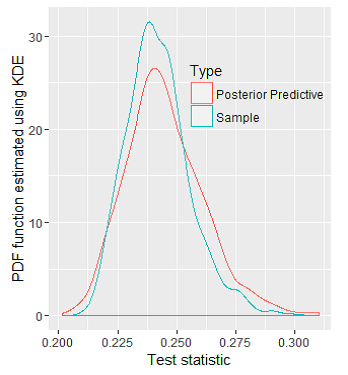
\includegraphics[width=\textwidth]{mainmatter/chapter_6_blood_donor/ppc_1comp.png}
        \caption{\label{fig : ppc_blood_donor_1comp}\#Components fitted = 1}
	\end{subfigure}
	\begin{subfigure}[b]{0.4\textwidth}
		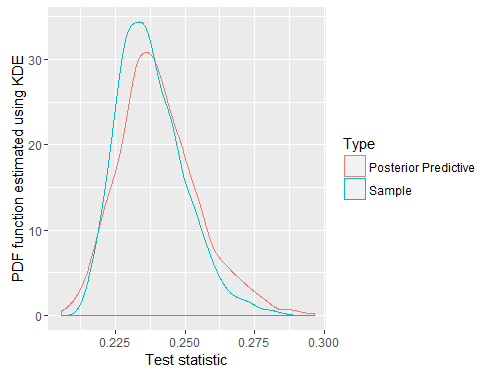
\includegraphics[width=\textwidth]{mainmatter/chapter_6_blood_donor/ppc_2comp.png}	
          \caption{\label{fig : ppc_blood_donor_2comp}\#Components fitted = 2}
	\end{subfigure}
	\caption{PDF function of $T(\boldsymbol{\tilde{r}})$ for underfitted/rightly fitted models applied to the blood donor data set.}
	\label{fig : ppc_blood_donor_underfitted}    
\end{figure} 

\begin{figure}[!htb]
\centering
\captionsetup{justification=centering}
\begin{subfigure}[b]{0.4\textwidth}
		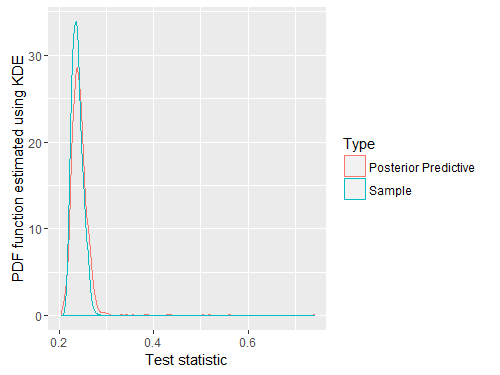
\includegraphics[width=\textwidth]{mainmatter/chapter_6_blood_donor/ppc_3comp.png}	
          \caption{\label{fig : ppc_blood_donor_3comp}\#Components fitted = 3}
	\end{subfigure}
	\begin{subfigure}[b]{0.4\textwidth}
		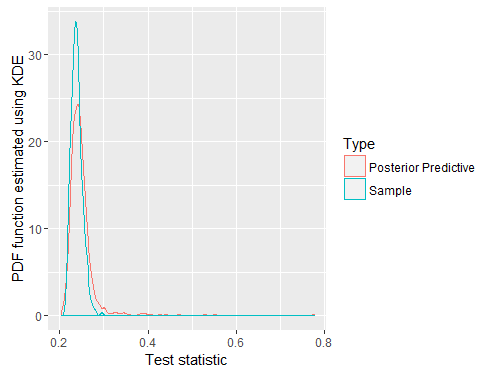
\includegraphics[width=\textwidth]{mainmatter/chapter_6_blood_donor/ppc_4comp.png}	
          \caption{\label{fig : ppc_blood_donor_4comp}\#Components fitted = 4}
	\end{subfigure}
	\begin{subfigure}[b]{0.4\textwidth}
		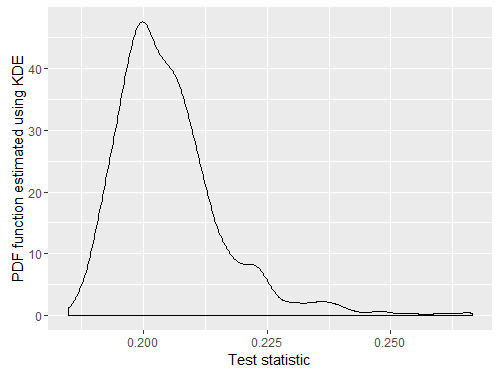
\includegraphics[width=\textwidth]{mainmatter/chapter_6_blood_donor/ppc_5comp.png}	
          \caption{\label{fig : ppc_blood_donor_5comp}\#Components fitted = 5}
	\end{subfigure}
	
	\caption{PDF function of $T(\boldsymbol{\tilde{r}})$ for overfitted models applied to the blood donor data set.}
	\label{fig : ppc_blood_donor_overfitted}    
\end{figure} 

\begin{table}[!htb]
\centering
\captionsetup{justification=centering}
\caption{PPP values for the various models fitted to the blood donor data set.}
\label{table : ppp_blood_donor}
\begin{tabular}{@{}rrrrrrrrr@{}}
\toprule
\# Components fitted & 1 & 2 & 3 & 4 & 5\\ \midrule
PPP Value & 0.619 & 0.591 & 0.677 & 0.701 & 0.758\\ \bottomrule
\end{tabular}
\end{table}

\section{Parameter estimates for the model with 2 components in mixture}
Table \ref{table : bhtge_blooddonor_2comp} shows the parameter estimates for the component densities of the mixture of random effects. Further, figure \ref{fig : eta_blood_donor} to figure \ref{fig : cov_blood_donor} show the posterior densities of the weight distribution, mean of the component densities and covariance parameters $\sigma^2_\text{Intercept}$, $\sigma^2_\text{Slope}$, $\sigma_\text{Intercept, Slope}$ which form the covariance matrix of component densities. For weight distribution $\boldsymbol{\eta}$ if we consider the mean of the posterior distributions then the weight distribution ratio for the components is 1:3. Secondly we can see that the posterior densities for location parameters for slope have a slight overlap but that is not the case with random intercept.\\

The first component in the mixture corresponds to the group for which the baseline random component of Hemoglobin is low and and the second component corresponds to the group for which the baseline random component of Hemoglobin is higher. However for the second group the slope is more negative suggesting that relative to group 1 an average subject from group 2 has a more rapid decrease in Hemoglobin levels with frequent donations. Lastly, within group 2 a person who begins with a higher baseline Hemoglobin level, is likely to have a more rapid decrease in Hemoglobin levels with donations. However within group 1 such intra subject difference cannot be generalized because 95\% HPDI for the correlation between random intercept and random slope is [-0.847, 0.980].\\

As for the fixed effects, we can see that subjects with higher age tend to have a lower Hb. Also during hot seasons the Hb levels are lower than in cold seasons. Both of these findings are consistent with the findings of \citet{nasserinejad_predicting_2013,nasserinejad_prevalence_2015,nasserinejad_prediction_2016}. We did not discuss the other fixed effects as the corresponding covariates also interact with other covariates in the model.

\begin{table}[htb]
\centering
\captionsetup{justification=centering}
\caption{Bayesian parameter estimates for the model with 2 components in the mixture of random effects, applied to the Blood donor data set.}
\label{table : bhtge_blooddonor_2comp}
\begin{tabular}{@{}lrrr@{}}
\toprule
Fixed Effects ($\beta$) & Mean & Median & 95\% HPDI \\ \midrule
Age &  -0.07 & -0.07 & -0.118, -0.024\\
TSPD & -0.038 & -0.038 & -0.066, -0.009\\
Season (Hot) & -0.081 & -0.081 & -0.113, -0.05\\
Donate (TRUE) & 0.160 & 0.159 & 0.091, 0.234\\
\#donationLast2Years * TSPD & 0.020 & 0.020 & 0.008, 0.030\\
\#donationLast2Years * Donate & 4.738 & 4.746 & 2.812, 6.733\\
$\text{\#donationLast2Years}^2$  & -48.360 & -48.256 & -76.647, -18.457\\ \bottomrule
\end{tabular}

\begin{tabular}{@{}lrrr@{}}
\toprule
Component Parameters & Mean & Median & 95\% HPDI \\ \midrule
$\eta_1$ & 0.275 & 0.265 & 0.137, 0.484\\
$\eta_2$ & 0.725 & 0.735 & 0.516, 0.863\\

$b_\text{Intercept-1}^C$ & 90.213 & 90.191 & 88.657, 91.67\\
$b_\text{Slope-1}^C$ & -4.835 & -4.896 & -8.626, -0.827\\

$b_\text{Intercept-2}^C$ & 95.645 & 95.578 & 94.246, 97.339\\
$b_\text{Slope-2}^C$ & -8.676 & -8.627 & -12.365, -5.386\\

$\sigma^2_\text{Intercept-1}$ & 2.108 & 1.562 & 0.067, 5.65\\
$\sigma_{\text{Intercept-1}, \text{Slope-1}}$ & 0.538 & 0.245 & -2.571, 5.403\\
$\rho_{\text{Intercept-1}, \text{Slope-1}}$ & 0.202 & 0.334 & -0.847, 0.980\\
$\sigma^2_\text{Slope-1}$ & 1.975 & 0.927 & 0.069, 7.579\\

$\sigma^2_\text{Intercept-2}$ & 18.176 & 18.146 & 11.677, 25.416\\
$\sigma_{\text{Intercept-2}, \text{Slope-2}}$ & -14.542 & -14.441 & -24.496, -5.069\\
$\rho_{\text{Intercept-2}, \text{Slope-2}}$ & -0.479 & -0.492 & -0.69, -0.252\\
$\sigma^2_\text{Slope-2}$ & 49.437 & 48.584 & 31.177, 72.200\\ \bottomrule
\end{tabular}

\begin{tabular}{@{}lrrr@{}}
\toprule
Variance Parameters & Mean & Median & 95\% HPDI \\ \midrule
$\sigma^2$ & 0.202 & 0.202 & 0.192, 0.212\\ \bottomrule
\end{tabular}
\end{table}

\begin{figure}[!htb]
\centering
\captionsetup{justification=centering}
\begin{subfigure}[b]{0.4\textwidth}
		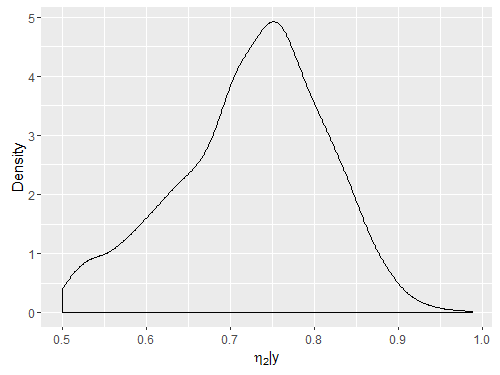
\includegraphics[width=\textwidth]{mainmatter/chapter_6_blood_donor/eta1.png}
        \caption{\label{fig : eta_blood_donor_1} Posterior $p(\eta_1|\boldsymbol{y})$}
	\end{subfigure}
	\begin{subfigure}[b]{0.4\textwidth}
		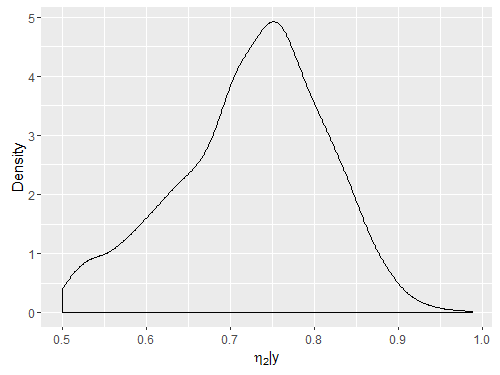
\includegraphics[width=\textwidth]{mainmatter/chapter_6_blood_donor/eta2.png}	
          \caption{\label{fig : eta_blood_donor_2}Posterior $p(\eta_2|\boldsymbol{y})$}
	\end{subfigure}	
	\caption{Posterior densities of the weight distribution for the components of the mixture of random effects for the blood donor data set.}
	\label{fig : eta_blood_donor}    
\end{figure} 

\begin{figure}[!htb]
\centering
\captionsetup{justification=centering}
\begin{subfigure}[b]{0.4\textwidth}
		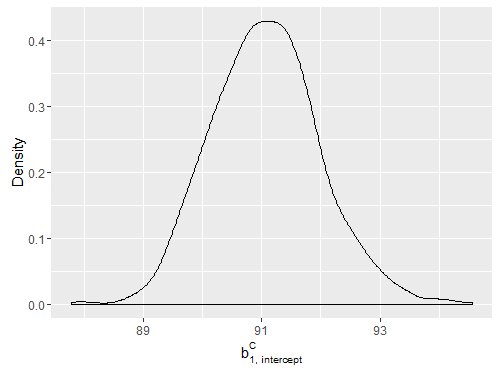
\includegraphics[width=\textwidth]{mainmatter/chapter_6_blood_donor/b11.png}
        \caption{\label{fig : mu_blood_donor_11}Posterior $p(b_\text{Intercept-1}^C|\boldsymbol{y})$}
	\end{subfigure}
	\begin{subfigure}[b]{0.4\textwidth}
		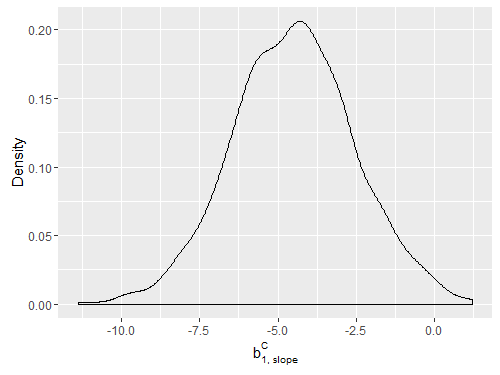
\includegraphics[width=\textwidth]{mainmatter/chapter_6_blood_donor/b12.png}	
          \caption{\label{fig : mu_blood_donor_12}Posterior $p(b_\text{Slope-1}^C|\boldsymbol{y})$}
	\end{subfigure}
	\begin{subfigure}[b]{0.4\textwidth}
		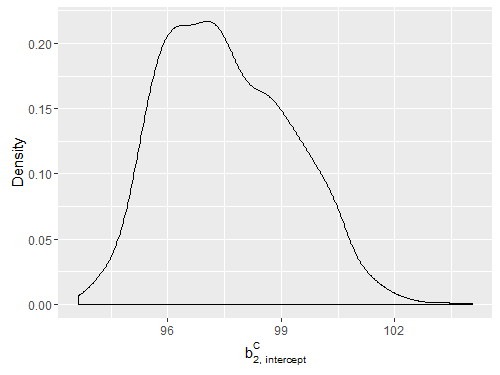
\includegraphics[width=\textwidth]{mainmatter/chapter_6_blood_donor/b21.png}	
          \caption{\label{fig : mu_blood_donor_21}Posterior $p(b_\text{Intercept-2}^C|\boldsymbol{y})$}
	\end{subfigure}	
	\begin{subfigure}[b]{0.4\textwidth}
		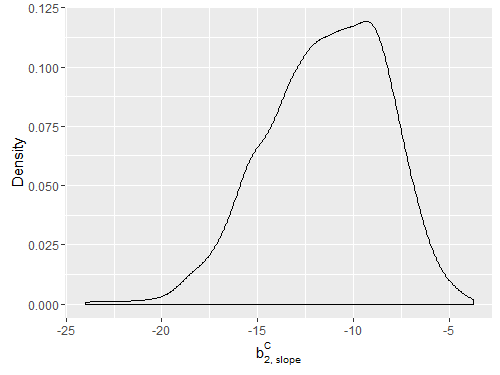
\includegraphics[width=\textwidth]{mainmatter/chapter_6_blood_donor/b22.png}	
          \caption{\label{fig : mu_blood_donor_22}Posterior $p(b_\text{Slope-2}^C|\boldsymbol{y})$}
	\end{subfigure}	
	\caption{Posterior densities of the location parameters for the components of the mixture of random effects for the blood donor data set.}
	\label{fig : mu_blood_donor}    
\end{figure} 

\begin{figure}[!htb]
\centering
\captionsetup{justification=centering}
\begin{subfigure}[b]{0.4\textwidth}
		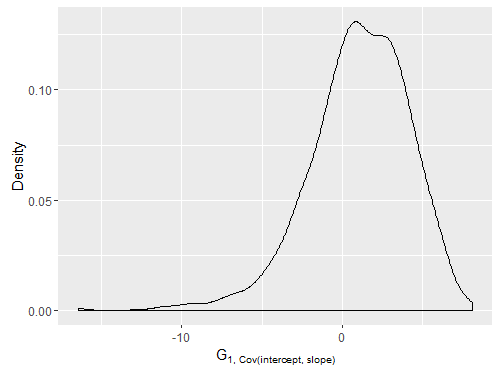
\includegraphics[width=\textwidth]{mainmatter/chapter_6_blood_donor/G11_1.png}
        \caption{\label{fig : cov_blood_donor_11_1}Posterior $p(\sigma^2_\text{Intercept-1}| \boldsymbol{y})$}
	\end{subfigure}
	\begin{subfigure}[b]{0.4\textwidth}
		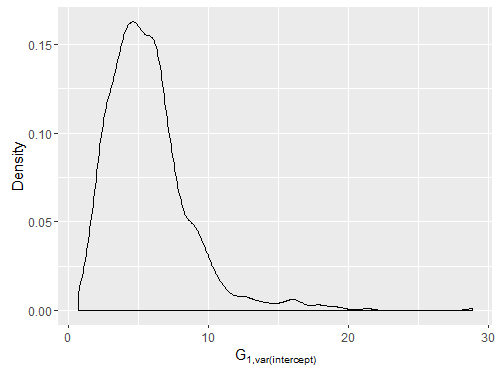
\includegraphics[width=\textwidth]{mainmatter/chapter_6_blood_donor/G12_1.png}	
          \caption{\label{fig : cov_blood_donor_12_1}Posterior $p(\sigma_{\text{Intercept-1}, \text{Slope-1}} | \boldsymbol{y})$}
	\end{subfigure}
	\begin{subfigure}[b]{0.4\textwidth}
		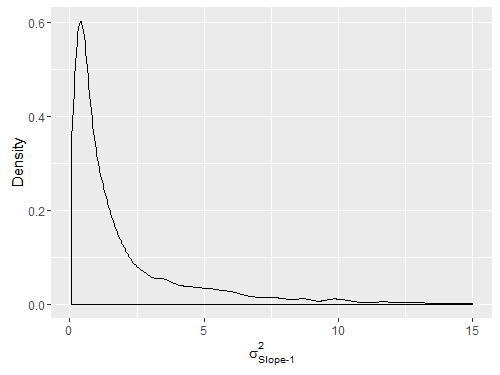
\includegraphics[width=\textwidth]{mainmatter/chapter_6_blood_donor/G22_1.png}	
          \caption{\label{fig : cov_blood_donor_22_1}Posterior $p(\sigma^2_\text{Slope-1}| \boldsymbol{y})$}
	\end{subfigure}	
	\begin{subfigure}[b]{0.4\textwidth}
		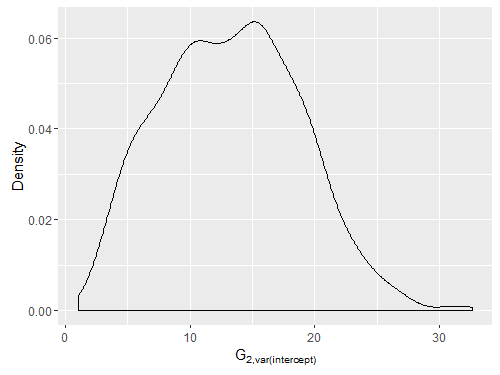
\includegraphics[width=\textwidth]{mainmatter/chapter_6_blood_donor/G11_2.png}
        \caption{\label{fig : cov_blood_donor_11_2}Posterior $p(\sigma^2_\text{Intercept-2}| \boldsymbol{y})$}
	\end{subfigure}
	\begin{subfigure}[b]{0.4\textwidth}
		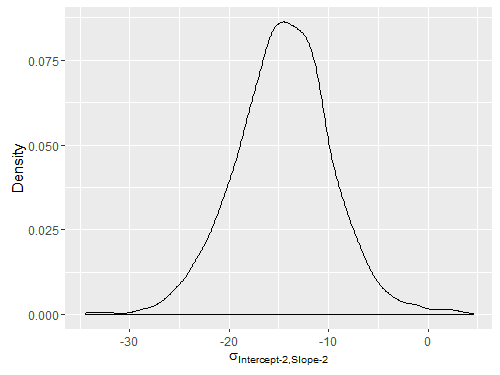
\includegraphics[width=\textwidth]{mainmatter/chapter_6_blood_donor/G12_2.png}	
          \caption{\label{fig : cov_blood_donor_12_2}Posterior $p(\sigma_{\text{Intercept-2}, \text{Slope-2}} | \boldsymbol{y})$}
	\end{subfigure}
	\begin{subfigure}[b]{0.4\textwidth}
		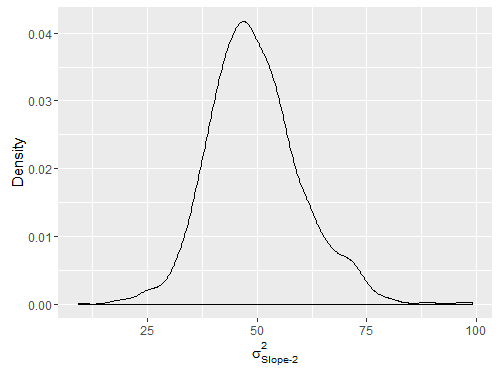
\includegraphics[width=\textwidth]{mainmatter/chapter_6_blood_donor/G22_2.png}	
          \caption{\label{fig : cov_blood_donor_22_2}Posterior $p(\sigma^2_\text{Slope-2}| \boldsymbol{y})$}
	\end{subfigure}	

	\caption{Posterior densities of the variance covariance parameters for the components of the mixture of random effects for the blood donor data set.}
	\label{fig : cov_blood_donor}    
\end{figure} 
\chapter{Conclusion}
\label{ch : conclusion}

\todo[inline]{Write something here}


% Appendices should go here
\appendix

% backmater => mainly references
\backmatter
\printbibliography
\cleardoublepage


\includepdf[pages={1}]{coverpages/backpage/backpage.pdf}
\end{document}
